% Options for packages loaded elsewhere
\PassOptionsToPackage{unicode}{hyperref}
\PassOptionsToPackage{hyphens}{url}
\PassOptionsToPackage{dvipsnames,svgnames,x11names}{xcolor}
\documentclass[
  english,
  10pt,
  a4paper,
]{article}
\usepackage{xcolor}
\usepackage[top=22mm,bottom=20mm,left=18mm,right=18mm]{geometry}
\usepackage{amsmath,amssymb}
\setcounter{secnumdepth}{-\maxdimen} % remove section numbering
\usepackage{iftex}
\ifPDFTeX
  \usepackage[T1]{fontenc}
  \usepackage[utf8]{inputenc}
  \usepackage{textcomp} % provide euro and other symbols
\else % if luatex or xetex
  \usepackage{unicode-math} % this also loads fontspec
  \defaultfontfeatures{Scale=MatchLowercase}
  \defaultfontfeatures[\rmfamily]{Ligatures=TeX,Scale=1}
\fi
\usepackage{lmodern}
\ifPDFTeX\else
  % xetex/luatex font selection
\fi
% Use upquote if available, for straight quotes in verbatim environments
\IfFileExists{upquote.sty}{\usepackage{upquote}}{}
\IfFileExists{microtype.sty}{% use microtype if available
  \usepackage[]{microtype}
  \UseMicrotypeSet[protrusion]{basicmath} % disable protrusion for tt fonts
}{}
\makeatletter
\@ifundefined{KOMAClassName}{% if non-KOMA class
  \IfFileExists{parskip.sty}{%
    \usepackage{parskip}
  }{% else
    \setlength{\parindent}{0pt}
    \setlength{\parskip}{6pt plus 2pt minus 1pt}}
}{% if KOMA class
  \KOMAoptions{parskip=half}}
\makeatother
\usepackage{longtable,booktabs,array}
\usepackage{caption}
\captionsetup[table]{skip=6pt}
\newcounter{none} % for unnumbered tables
\usepackage{calc} % for calculating minipage widths
% Correct order of tables after \paragraph or \subparagraph
\usepackage{etoolbox}
\makeatletter
\patchcmd\longtable{\par}{\if@noskipsec\mbox{}\fi\par}{}{}
\makeatother
\ifLuaTeX
\usepackage[bidi=basic,shorthands=off]{babel}
\else
\usepackage[bidi=default,shorthands=off]{babel}
\fi
\ifLuaTeX
  \usepackage{selnolig} % disable illegal ligatures
\fi
\setlength{\emergencystretch}{3em} % prevent overfull lines
\providecommand{\tightlist}{%
  \setlength{\itemsep}{0pt}\setlength{\parskip}{0pt}}
% ---- Çılgın Kurye document theme: same look as the CSE 396 project proposal ----
% Compile with XeLaTeX (also works on Overleaf). Fonts: TeX Gyre Termes (Times), DejaVu Sans Mono.
\usepackage{fontspec}
\setmainfont{texgyretermes}[Extension=.otf, UprightFont=*-regular, BoldFont=*-bold, ItalicFont=*-italic, BoldItalicFont=*-bolditalic]
\setsansfont{texgyreheros}[Extension=.otf, UprightFont=*-regular, BoldFont=*-bold, ItalicFont=*-italic, BoldItalicFont=*-bolditalic]
\setmonofont{DejaVuSansMono}[Extension=.ttf, UprightFont=*, BoldFont=*-Bold, ItalicFont=*-Oblique, BoldItalicFont=*-BoldOblique, Scale=0.80]
\setmathfont{texgyretermes-math.otf}

\usepackage{xcolor}
\definecolor{ckblue}{HTML}{1F3A5F}
\definecolor{cklight}{HTML}{E8EEF5}
\definecolor{ckgrey}{HTML}{F2F2F2}
\definecolor{ckline}{HTML}{555555}
\definecolor{shadecolor}{HTML}{F4F5F7}

% Headings as in the proposal: serif, bold; subsections bold italic. Numbers are part of the heading text.
\setcounter{secnumdepth}{0}
\usepackage{titlesec}
\titleformat{\section}{\rmfamily\Large\bfseries}{}{0pt}{}
\titleformat{\subsection}{\rmfamily\large\bfseries\itshape}{}{0pt}{}
\titleformat{\subsubsection}{\rmfamily\normalsize\bfseries}{}{0pt}{}
\titlespacing*{\section}{0pt}{12pt}{4pt}
\titlespacing*{\subsection}{0pt}{8pt}{3pt}

% Header and footer (the first page has only the footer, like the proposal)
\usepackage{fancyhdr,lastpage}
\pagestyle{fancy}
\fancyhf{}
\fancyhead[L]{\footnotesize\itshape CSE 396 · Group 8 · Çılgın Kurye}
\fancyhead[R]{\footnotesize\itshape\ckmodule}
\fancyfoot[C]{\footnotesize Page \thepage\ of \pageref*{LastPage}}
\renewcommand{\headrulewidth}{0.4pt}
\setlength{\headheight}{14pt}
\fancypagestyle{ckfirst}{\fancyhf{}\renewcommand{\headrulewidth}{0pt}\fancyfoot[C]{\footnotesize Page \thepage\ of \pageref*{LastPage}}}

% Inline code: breaks only after . : ( , / _ and spaces, never inside a name
\usepackage[obeyspaces,spaces]{url}
\AtBeginDocument{%
  \renewcommand{\UrlBreaks}{\do\.\do\:\do\(\do\,\do\/\do\_\do\|}%
  \renewcommand{\UrlBigBreaks}{}%
  \renewcommand{\UrlNoBreaks}{}%
  \urlstyle{tt}}

% Tables: boxed grid as in the proposal, smaller text
\usepackage{etoolbox}
\AtBeginEnvironment{longtable}{\footnotesize\renewcommand{\arraystretch}{1.2}}
\setlength{\LTpre}{6pt}
\setlength{\LTpost}{8pt}
\setlength{\arrayrulewidth}{0.4pt}

% Code blocks: long lines wrap; diagrams stay in one piece
\usepackage{framed}
\usepackage{fvextra}
\RecustomVerbatimEnvironment{verbatim}{Verbatim}{fontsize=\footnotesize, breaklines}
\makeatletter
\@ifundefined{Shaded}{}{\renewenvironment{Shaded}{\begin{snugshade}}{\end{snugshade}}}
\@ifundefined{Highlighting}{}{\RecustomVerbatimEnvironment{Highlighting}{Verbatim}{commandchars=\\\{\}, fontsize=\footnotesize, breaklines, breakanywhere}}
\makeatother

% Figures drawn with TikZ
\usepackage{tikz}
\usetikzlibrary{arrows.meta,positioning,fit,calc,backgrounds,shapes.geometric}
\tikzset{
  ck/.style={font=\footnotesize, >={Stealth[length=5pt]}, line width=0.6pt},
  box/.style={draw=ckline, fill=white, rounded corners=2pt, align=center, inner sep=4pt, minimum height=7mm},
  mod/.style={box, fill=ckgrey},
  this/.style={box, fill=cklight, draw=ckblue, line width=0.9pt},
  group/.style={draw=ckline, dashed, rounded corners=3pt, inner sep=6pt},
  lbl/.style={font=\scriptsize, align=center, inner sep=1.5pt},
  msg/.style={->, draw=ckline},
}
\usepackage{caption}
\captionsetup[figure]{font=small, labelfont=bf, skip=4pt}
\newcommand{\ckfigure}[2]{\begin{figure}[htbp]\centering #1\caption{#2}\end{figure}}

\usepackage{enumitem}
\setlist{itemsep=1pt, topsep=3pt}
\setlength{\parskip}{4pt}
\setlength{\parindent}{0pt}
\raggedbottom
% ---- end of theme ----
\newcommand{\ckmodule}{Modules and Requirements}
\usepackage{graphicx}
\usepackage{bookmark}
\IfFileExists{xurl.sty}{\usepackage{xurl}}{} % add URL line breaks if available
\urlstyle{same}
% fallback for those not using the hyperref driver hyperxmp:
\makeatletter
\@ifundefined{xmpquote}{\newcommand{\xmpquote}[1]{#1}}{}
\makeatother
\hypersetup{
  pdftitle={Çılgın Kurye: Modules and Requirements},
  pdflang={en},
  colorlinks=true,
  linkcolor={black},
  filecolor={Maroon},
  citecolor={Blue},
  urlcolor={black},
  pdfcreator={LaTeX}}

\title{M1 Game Server and Rules --- Module Documentation}
\author{}
\date{}


% ---- colours and drawings ----
% ---- colours ----
\definecolor{srv}{HTML}{2E6FB7}\colorlet{srvL}{srv!15}
\definecolor{cli}{HTML}{2E9E5B}\colorlet{cliL}{cli!15}
\definecolor{adm}{HTML}{E08A1E}\colorlet{admL}{adm!18}
\definecolor{brd}{HTML}{7B4FB3}\colorlet{brdL}{brd!15}
\definecolor{tcpc}{HTML}{1F5FA8}
\definecolor{udpc}{HTML}{D9531E}
\definecolor{obs}{HTML}{D7263D}
\definecolor{tA}{HTML}{00A6D6}
\definecolor{tB}{HTML}{3BB273}
\definecolor{tC}{HTML}{F2C14E}
\definecolor{tD}{HTML}{9B5DE5}

% ---- styles ----
\tikzset{
  nb/.style={rounded corners=3pt, line width=0.9pt, align=center, inner sep=4pt, minimum height=9mm, font=\footnotesize},
  sv/.style={nb, draw=srv, fill=srvL},
  cl/.style={nb, draw=cli, fill=cliL},
  ad/.style={nb, draw=adm, fill=admL},
  bd/.style={nb, draw=brd, fill=brdL},
  hwb/.style={nb, draw=black!50, fill=black!5},
  tcpa/.style={draw=tcpc, line width=1.5pt},
  udpa/.style={draw=udpc, line width=1.5pt, dash pattern=on 5pt off 2.5pt},
  inna/.style={draw=black!55, line width=1pt},
  al/.style={font=\scriptsize, fill=white, inner sep=1.2pt, rounded corners=1pt},
  grp/.style={draw=black!35, dashed, rounded corners=5pt, inner sep=7pt},
  glbl/.style={font=\scriptsize\bfseries, text=black!65},
  hl/.style={line width=2.6pt},
  st/.style={nb, rounded corners=8pt, minimum width=24mm},
  co/.style={draw=black!60, line width=0.5pt},
  cot/.style={font=\scriptsize, align=left, text=black!80},
}

% ---- system map; argument = module to highlight (M1 ... M8, or none) ----
\newcommand{\systemmap}[1]{%
\tikzset{M1/.style={},M2/.style={},M3/.style={},M4/.style={},M5/.style={},M6/.style={},M7/.style={},M8/.style={},none/.style={}}%
\tikzset{#1/.style={hl}}%
\begin{tikzpicture}[ck]
\node[cl, M5, minimum width=27mm] (m5) at (0,3) {\textbf{M5}\\Player phones};
\node[ad, M6, minimum width=27mm] (m6) at (0,0.4) {\textbf{M6}\\Admin panel};
\node[sv, M2, minimum width=27mm, minimum height=38mm] (m2) at (4.6,1.7) {\textbf{M2}\\Network\\and sync};
\node[sv, M1, minimum width=27mm, minimum height=38mm] (m1) at (8.4,1.7) {\textbf{M1}\\Game server\\and rules};
\node[sv, M3, minimum width=25mm] (m3) at (12,2.8) {\textbf{M3}\\Physics};
\node[sv, M4, minimum width=25mm] (m4) at (12,0.6) {\textbf{M4}\\Traffic and AI};
\node[grp, fit=(m2)(m1)(m3)(m4)] (pc) {};
\node[glbl, anchor=south west] at (pc.north west) {MAIN COMPUTER};
\node[bd, M7, minimum width=27mm] (m7) at (4.6,-2.7) {\textbf{M7}\\ESP32 software};
\node[bd, M8, minimum width=27mm] (m8) at (8.4,-2.7) {\textbf{M8}\\LED engine};
\node[hwb, minimum width=25mm] (led) at (12,-2.7) {344 LEDs};
\node[hwb, minimum width=27mm] (sm) at (4.6,-4.4) {Sensor and\\4 motors};
\node[grp, fit=(m7)(m8)(led)(sm)] (bb) {};
\node[glbl, anchor=north east] at (bb.south east) {LED CITY BOARD};
\draw[tcpa, <->] (m5.east) -- node[al]{WebSocket} (m5.east -| m2.west);
\draw[tcpa, <->] (m6.east) -- node[al]{WebSocket} (m6.east -| m2.west);
\draw[tcpa, <->] ([xshift=-6mm]m7.north) -- node[al]{TCP} ([xshift=-6mm]m2.south);
\draw[udpa, <->] ([xshift=6mm]m7.north) -- node[al]{UDP} ([xshift=6mm]m2.south);
\draw[inna, <->] (m2) -- (m1);
\draw[inna, <->] (m1.east |- m3) -- (m3);
\draw[inna, <->] (m1.east |- m4) -- (m4);
\draw[inna, ->] (m7) -- node[al]{state} (m8);
\draw[inna, ->] (m8) -- (led);
\draw[inna, <->] (m7) -- (sm);
\draw[tcpa] (-1.3,-6.0) -- ++(0.9,0) node[right, font=\scriptsize]{TCP: every message arrives, in order};
\draw[udpa] (4.0,-6.0) -- ++(0.9,0) node[right, font=\scriptsize]{UDP: fast, the newest message wins};
\draw[inna] (9.3,-6.0) -- ++(0.9,0) node[right, font=\scriptsize]{inside one program or chip};
\end{tikzpicture}}

% ---- LED board seen from above (6 x 6 roads, 1 unit = 10 cm) ----
\newcommand{\boardbase}{%
\fill[black!88, rounded corners=3pt] (-0.5,-0.5) rectangle (5.5,5.5);
\foreach \i in {0,...,4}{\foreach \j in {0,...,4}{%
  \fill[black!60] (\i+0.13,\j+0.13) rectangle (\i+0.87,\j+0.87);
  \fill[black!22] (\i+0.24,\j+0.24) rectangle (\i+0.52,\j+0.52);
  \fill[black!30] (\i+0.56,\j+0.30) rectangle (\i+0.78,\j+0.62);
  \fill[black!38] (\i+0.28,\j+0.58) rectangle (\i+0.66,\j+0.78);}}
\foreach \i in {0,...,5}{%
  \draw[black, line width=4.5pt] (\i,-0.05) -- (\i,5.05);
  \draw[black, line width=4.5pt] (-0.05,\i) -- (5.05,\i);}
\foreach \i in {0,...,5}{\foreach \k in {0,...,30}{%
  \fill[black!55] (\i,\k/6) circle (0.025);
  \fill[black!55] (\k/6,\i) circle (0.025);}}
\foreach \x/\y/\c in {0/4/tA, 4/4/tB, 0/0/tC, 4/0/tD}{%
  \fill[\c!30!black!60] (\x+0.13,\y+0.13) rectangle (\x+0.87,\y+0.87);
  \fill[\c] (\x+0.3,\y+0.3) rectangle (\x+0.7,\y+0.7);
  \fill[white] (\x+0.4,\y+0.5) circle (0.05); \fill[white] (\x+0.6,\y+0.5) circle (0.05);}}
\newcommand{\nmark}[3]{\node[circle, fill=yellow!85!orange, draw=black, line width=0.4pt, inner sep=0.6pt, minimum size=3.6mm, font=\tiny\bfseries] at (#1,#2) {#3};}
\newcommand{\bike}[4]{%
\fill[#3!35] ($(#1,#2)+(#4:0.40)$) circle (0.05);
\fill[#3!65] ($(#1,#2)+(#4:0.21)$) circle (0.075);
\fill[#3, draw=white, line width=0.4pt] (#1,#2) circle (0.12);}
\newcommand{\dpoint}[3]{\draw[#3!50, line width=0.8pt] (#1,#2) circle (0.26); \draw[#3, line width=1.4pt] (#1,#2) circle (0.16); \fill[#3] (#1,#2) circle (0.07);}
\newcommand{\heavy}[2]{\draw[obs!60!black, line width=4pt] (#1) -- (#2); \draw[obs, line width=4pt, dash pattern=on 3pt off 5pt] (#1) -- (#2);}
\newcommand{\roadwork}[2]{\draw[obs, line width=4pt] (#1) -- (#2);}
\newcommand{\accident}[2]{\draw[obs, line width=4pt] (#1) -- (#2); \draw[white, line width=4pt, dash pattern=on 2.5pt off 3.5pt] (#1) -- (#2);}
\newcommand{\puddle}[2]{\draw[cyan!35, line width=4pt] (#1) -- (#2); \draw[white, line width=1.6pt, dash pattern=on 1pt off 2.5pt] (#1) -- (#2);}
\newcommand{\findme}[2]{\fill[white, opacity=0.25] (#1,#2) circle (0.36); \fill[white, opacity=0.5] (#1,#2) circle (0.24); \fill[white] (#1,#2) circle (0.13);}

% ---- phone game screen (7 x 3.4 units) ----
\newcommand{\phonemock}{%
\fill[black!85, rounded corners=9pt] (-0.3,-0.3) rectangle (7.3,3.7);
\fill[cyan!20] (0,1.7) rectangle (7,3.4);
\fill[cli!14] (0,0) rectangle (7,1.7);
\filldraw[fill=srv!30, draw=srv!70!black] (0.2,1.5) rectangle (1.0,3.0);
\filldraw[fill=adm!35, draw=adm!70!black] (1.1,1.6) rectangle (1.8,2.4);
\filldraw[fill=brd!30, draw=brd!70!black] (1.9,1.65) -- (2.6,1.65) -- (2.6,2.2) -- (2.25,2.5) -- (1.9,2.2) -- cycle;
\filldraw[fill=adm!35, draw=adm!70!black] (4.5,1.65) rectangle (5.1,2.3);
\filldraw[fill=srv!30, draw=srv!70!black] (5.2,1.55) rectangle (6.0,3.1);
\filldraw[fill=cli!35, draw=cli!70!black] (6.1,1.6) rectangle (6.85,2.6);
\fill[brown!60!black] (4.17,1.6) rectangle (4.23,1.8); \fill[cli!70!black] (4.2,1.95) circle (0.18);
\fill[black!55] (1.8,0) -- (5.2,0) -- (3.75,1.7) -- (3.25,1.7) -- cycle;
\draw[white, line width=0.8pt, dash pattern=on 4pt off 4pt] (3.5,0) -- (3.5,1.7);
\filldraw[fill=black!15, draw=black!70] (3.62,1.12) rectangle (3.88,1.32);
\fill[obs] (3.05,1.22) -- (3.15,1.48) -- (3.25,1.22) -- cycle;
\fill[black!85] (3.43,0.08) rectangle (3.57,0.3);
\fill[tA] (3.3,0.28) rectangle (3.7,0.6);
\fill[brown!65] (3.34,0.6) rectangle (3.66,0.82);
\fill[tA!60!black] (3.5,0.95) circle (0.13);
\node[fill=black!70, text=white, rounded corners=2pt, font=\scriptsize\bfseries, inner sep=2pt] at (3.5,3.15) {2:41};
\foreach \c/\s/\x in {tA/120/0.35,tB/95/0.95,tC/140/1.55,tD/80/2.15}
  \node[fill=\c, text=white, font=\tiny\bfseries, rounded corners=1pt, inner sep=1.5pt, minimum width=5mm] at (\x,3.15) {\s};
\fill[white, opacity=0.9] (6.45,2.85) circle (0.38); \draw[black!60] (6.45,2.85) circle (0.38);
\draw[-{Stealth[length=5pt]}, line width=1.8pt, obs] (6.45,2.85) ++(230:0.2) -- ++(50:0.5);
\fill[white, opacity=0.85] (0.55,0.5) circle (0.32); \fill[black!70] (0.43,0.5) -- (0.65,0.63) -- (0.65,0.37) -- cycle;
\fill[white, opacity=0.85] (1.4,0.5) circle (0.32); \fill[black!70] (1.52,0.5) -- (1.3,0.63) -- (1.3,0.37) -- cycle;
\node[fill=obs!80, text=white, rounded corners=3pt, font=\tiny\bfseries, minimum width=8mm, minimum height=6mm] at (5.6,0.5) {Brake};
\node[fill=cli, text=white, rounded corners=3pt, font=\tiny\bfseries, minimum width=8mm, minimum height=8mm] at (6.5,0.6) {Gas};
\node[fill=tC, text=black, rounded corners=3pt, font=\tiny\bfseries, minimum width=9mm, minimum height=5mm] at (6.15,1.45) {Deliver};
\node[fill=white, text=black, rounded corners=3pt, font=\tiny\bfseries, minimum width=9mm, minimum height=5mm] at (0.9,1.45) {Find me};}

% ---- side cut of the board (14 units wide) ----
\newcommand{\boardside}{%
\fill[brown!20] (-0.6,-0.35) rectangle (14.6,0);
\foreach \x/\h/\c in {1.0/0.7/black!18, 2.2/1.1/black!22, 4.6/1.9/black!25, 5.8/2.6/black!28, 7.4/2.2/black!25, 8.6/1.6/black!22, 10.9/1.0/black!18}
  \filldraw[fill=\c, draw=black!45] (\x,1.5) rectangle (\x+0.9,1.5+\h);
\filldraw[fill=tB!35, draw=tB!70!black] (12.4,1.5) rectangle (13.4,2.3);
\fill[black!70, rounded corners=1pt] (0.5,0) rectangle (1.1,0.9);
\fill[black!70, rounded corners=1pt] (12.9,0) rectangle (13.5,0.9);
\filldraw[fill=brown!45, draw=brown!70!black] (0,0.9) rectangle (14,1.3);
\fill[black!80] (0,1.3) rectangle (14,1.38);
\foreach \x in {0.3,0.9,...,13.8} \fill[black!35] (\x,1.42) circle (0.06);
\foreach \x/\c in {3.3/tA, 3.9/tA, 6.9/obs, 7.5/obs, 10.5/tC} \fill[\c] (\x,1.42) circle (0.07);
\fill[white, opacity=0.55] (0,1.38) rectangle (14,1.52);
\filldraw[fill=brd!40, draw=brd] (2.3,0.35) rectangle (4.3,0.85);
\node[font=\tiny] at (3.3,0.6) {ESP32};
\filldraw[fill=brd, draw=brd!60!black] (6.75,0.62) rectangle (7.25,0.88);
\filldraw[fill=adm!60, draw=adm!70!black] (1.8,0.6) circle (0.24);
\filldraw[fill=adm!60, draw=adm!70!black] (12.2,0.6) circle (0.24);
\filldraw[fill=black!15, draw=black!50] (9.3,0.35) rectangle (10.9,0.85);
\node[font=\tiny] at (10.1,0.6) {Power};}

\begin{document}

% ---- table and list helpers ----
\newcolumntype{L}[1]{>{\raggedright\arraybackslash}p{\dimexpr#1\linewidth-2\tabcolsep-\arrayrulewidth\relax}}
\newcolumntype{C}[1]{>{\centering\arraybackslash}p{\dimexpr#1\linewidth-2\tabcolsep-\arrayrulewidth\relax}}
\newcommand{\ckdone}{\item[$\boxtimes$]}
\newcommand{\ckopen}{\item[$\square$]}
\newcommand{\mdot}{$\bullet$}
\newcounter{msec}
\newcounter{chap}
% ---- end of helpers ----
\newcommand{\msection}[1]{\stepcounter{msec}\subsection{\arabic{chap}.\arabic{msec} #1}}
\thispagestyle{ckfirst}
\begin{center}
{\bfseries GEBZE TECHNICAL UNIVERSITY\par}
{Computer Engineering Department\par}
{CSE 396 Module Documentation\par}
\vspace{8pt}
{\LARGE\bfseries Çılgın Kurye\par}
\vspace{3pt}
{\large\itshape Modules and requirements\par}
\vspace{6pt}
\textbf{Instructor:} Erkan Zergeroğlu\hspace{1.4em}\textbf{Company:} Board\&Byte\hspace{1.4em}\textbf{Group:} Group-8\hspace{1.4em}\textbf{Date:} 6 November 2026
\end{center}
\begin{center}\footnotesize\renewcommand{\arraystretch}{1.15}
\begin{tabular}{|p{0.27\linewidth}|p{0.15\linewidth}|p{0.27\linewidth}|p{0.15\linewidth}|}\hline
\textbf{Name} & \textbf{Student No.} & \textbf{Name} & \textbf{Student No.} \\ \hline
Tuğberk Akbulut & 230104004070 & Abdullatif Yılmaz & 230104004031 \\ \hline
Hasan Alperen Elmas & 1801042604 & Batuhan Yanar & 220104004059 \\ \hline
Ayşe Poyraz & 230104004085 & Berk Andaçgil & 230104004066 \\ \hline
Hasan Hüseyin Özdemir & 230104004048 & Muhib Taha Boy & 230104004165 \\ \hline
Selim Barut & 220104004046 & Umutcan Ocak & 220104004903 \\ \hline
\end{tabular}
\end{center}

\section{1. Project overview}

Çılgın Kurye is a multiplayer motorcycle courier game. Players play it in the web browser of their
own phones, so there is nothing to install. Up to 8 players play at the same time in 4 teams, and the
whole game runs on a server on one computer. Each player rides a motorcycle in a 3D city and carries
packages from the team's store to delivery points. The team with the most points after 5 minutes
wins.

The special part of the game is that the phone has no map. To find the delivery point, players must
look at the 60 × 60 cm city board on the table. LED strips in the roads of the board show all
motorcycles, delivery points and obstacles in real time. The players can also hit the board with
their hand to start an earthquake in the game. The admin computer is the control centre. During the
game the admin changes parameters and sees each change in three places: in the 3D city on the
phones, on the LED board and in live graphs. The computer, the phones and the board talk over Wi-Fi.

\begin{figure}[htbp]\centering
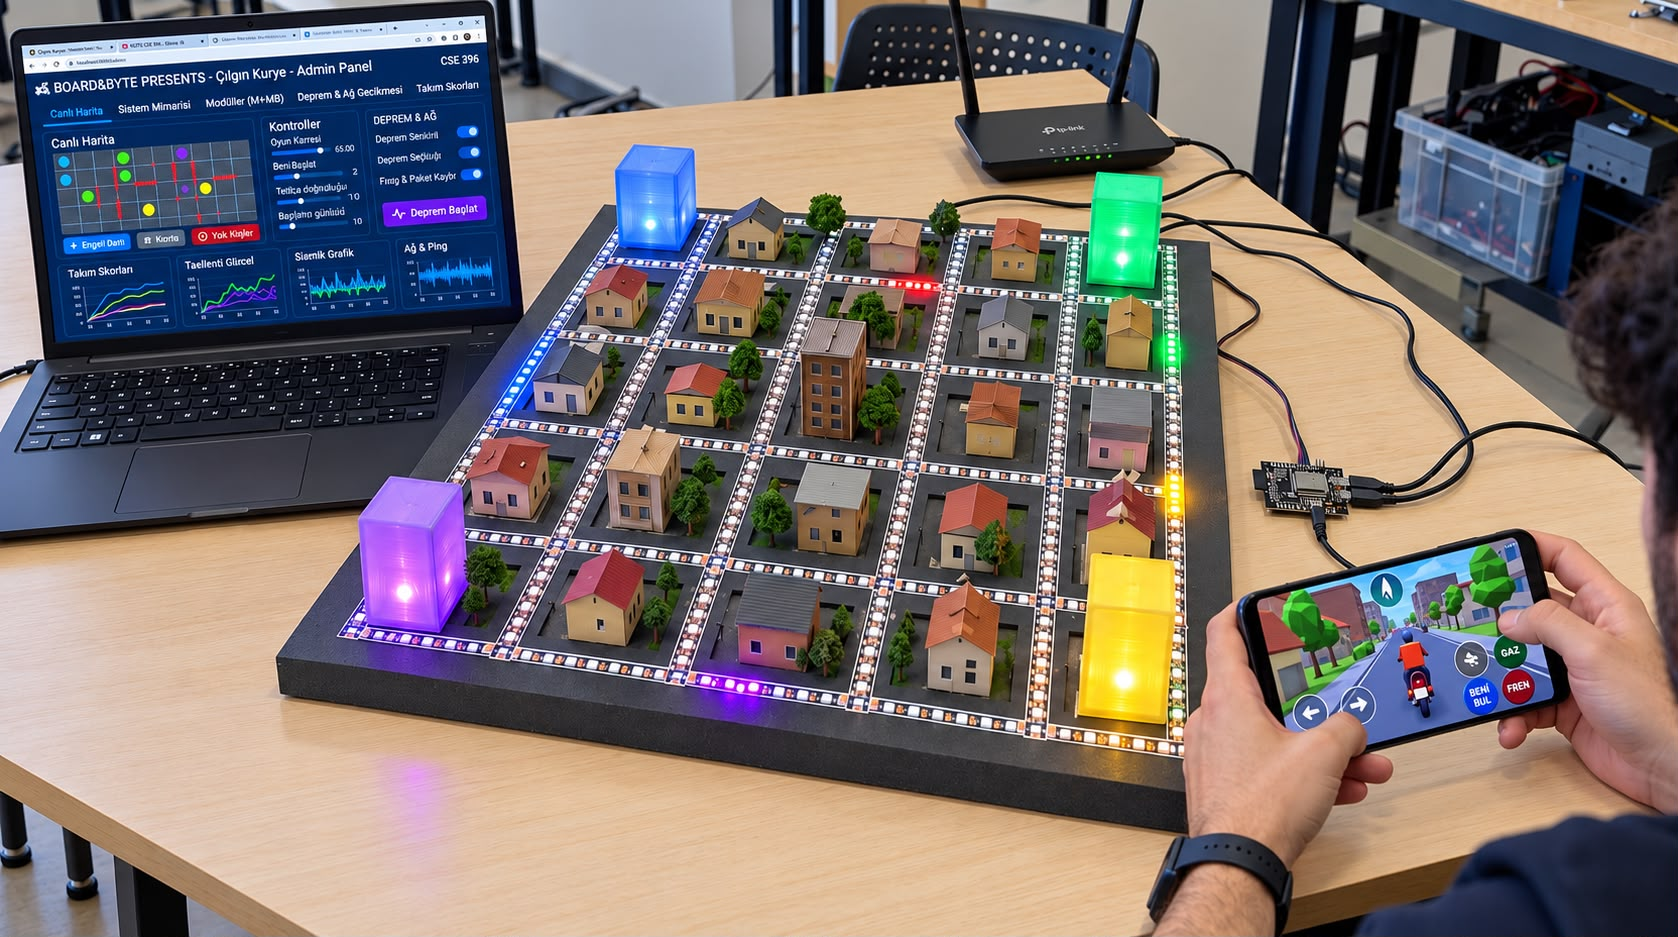
\includegraphics[width=0.80\linewidth]{target-system.png}
\caption{The target system: the LED city board, the admin screen and the game on a phone.}
\end{figure}

\section{2. System architecture}

The main computer runs one server program. Inside it, M1 runs the game, M3 moves the motorcycles,
M4 runs the traffic and the bots, and M2 does all the network work. This program makes every final
decision, so all players see the same game. The phones (M5) only send their buttons and draw the 3D
city. The admin page (M6) sends commands and shows graphs. In the LED board, the ESP32 runs the link
and the sensor (M7) on one core and the LED engine (M8) on the other core.

\begin{figure}[htbp]\centering
\systemmap{none}
\caption{The eight modules and the links between them.}
\end{figure}

We chose the protocol of each link with care. A web browser can only open a WebSocket for two-way
talk, so the phones and the admin page use WebSocket, which runs on TCP. The LED board uses two
channels. Messages that must never be lost go on TCP: the config, the vibrate commands for the
motors, the earthquake events and the status report. Data that comes many times per second goes on
UDP: the board state, the sensor samples and the delay probes. With UDP a lost packet is simply
replaced by the next one, so the LEDs never stop to wait.

\begin{figure}[htbp]\centering
\begin{tikzpicture}[ck]
\node[cl, minimum width=22mm] (a) at (0,0) {Player presses\\gas};
\node[cl, minimum width=22mm] (b) at (3.3,0) {Phone moves\\at once};
\node[sv, minimum width=22mm] (c) at (6.6,0) {M2 checks,\\M1 tick};
\node[sv, minimum width=22mm] (d) at (9.9,0) {State to\\everybody};
\node[cl, minimum width=22mm] (e) at (13.2,1.2) {Other phones\\draw it};
\node[ad, minimum width=22mm] (f) at (13.2,0) {Admin map\\and graphs};
\node[bd, minimum width=22mm] (g) at (13.2,-1.2) {LED dot\\moves};
\draw[inna,->] (a) -- (b);
\draw[tcpa,->] (b) -- (c);
\draw[inna,->] (c) -- (d);
\draw[tcpa,->] (d) -- (e.west);
\draw[tcpa,->] (d) -- (f);
\draw[udpa,->] (d) -- (g.west);
\end{tikzpicture}
\caption{One button press from the phone to every screen and to the board. Blue solid is TCP, orange dashed is UDP.}
\end{figure}

Five rules hold for the whole system. First, there is one authority: only M1 changes the game state,
and only inside a tick. Second, inputs are safe: phones send controls, never positions or scores,
and M2 checks every message before M1 sees it. Third, all modules use shared contract files for the
messages and one shared city plan, so the 3D city and the board always match. Fourth, each module
can be built and tested alone with fake data from its neighbours. Fifth, the inputs of every tick
go into a log, so a game can be played again exactly for testing.

\section{3. System requirements}

The table lists the requirements of the whole system. The last column shows the modules that meet
each requirement.

\begin{longtable}[]{|L{0.05}|L{0.16}|L{0.63}|L{0.16}|}
\hline \textbf{No} & \textbf{Requirement} & \textbf{Description} & \textbf{Modules} \\ \hline \endhead
R1 & Multiplayer game & At most 8 players in 4 teams (at most 2 per team); a game lasts at most 5 minutes. AI bots fill empty places; the team with the most delivery points wins. & M1 M2 M4 M5 \\ \hline
R2 & Delivery cycle & The player takes a package from the store; the server chooses a delivery point by travel time with the current obstacles; the point blinks on the board in the player's tone. The player delivers and returns to the store. The near / far chance is set per player by the admin. & M1 M4 M5 M8 \\ \hline
R3 & Driving and controls & Free driving, lane changes and passing obstacles; no reverse, U-turn by steering. Throttle, brake, left and right buttons on the phone. & M3 M5 \\ \hline
R4 & Collisions, falls, traffic & In a fast collision both players fall and wait a short penalty. NPC cars create real traffic; hitting a car, a building or an obstacle fast makes the player fall. Penalty time and traffic / obstacle density are admin parameters. & M1 M3 M4 \\ \hline
R5 & No map on the phone & The phone shows only a compass arrow to the delivery point (or back to the store); no distance and no roads. Players must look at the board. ``Find me'' lights the player's LED white for 1 s. & M1 M5 M8 \\ \hline
R6 & Obstacles & Four types: heavy traffic, road work, accident, water puddle. On the board red always means ``this road slows you down''; the pattern shows the type. The admin can change the effect of each type. & M1 M3 M4 M6 M8 \\ \hline
R7 & Earthquake mode & Starts by hitting the board by hand or with the admin button (vibration motors under the board); the sensor measures strength and approximate area. In the game the camera shakes, motorcycles fall and roads near the centre close; a shock wave spreads on the board. The strength is an admin parameter. & M1 M3 M5 M6 M7 M8 \\ \hline
R8 & Physical LED board & 60 × 60 cm, 6 roads in each direction (5 × 5 blocks), addressable LEDs on all roads, 3D-printed buildings, four stores with two RGB LEDs each in the corners; the ESP32 connects over Wi-Fi. The 3D city and the board are built from the same city plan. & M5 M7 M8 \\ \hline
R9 & Live admin panel & All parameters are changed during the game; the admin sees the change in three places: 3D simulation, LED board and live graphs. & M1 M2 M6 \\ \hline
R10 & Network and measurement & Computer, phones and board talk over Wi-Fi. The admin can add delay, packet loss and a frame-rate limit per player, and delay and loss on the board link; ping, packet loss and frame rate are measured live. & M2 M5 M6 M7 \\ \hline
R11 & Engineering requirements & The main computer makes all game decisions (single authority); the phone only sends controls and sees its own motorcycle at once (prediction). Inputs and outputs of every module are defined, and each module can be developed and tested with mock data. & M1--M8 \\ \hline
\end{longtable}

\section{4. Modules}

The project has eight modules on three sides: the server (M1--M4), the phone and admin pages (M5,
M6) and the physical board (M7, M8). Every module has at least 3 members, and every member works in
3 modules. So a module can go on even if one member leaves. An X in the second table means that the
member works in that module.

\begin{longtable}[]{|L{0.07}|L{0.28}|L{0.56}|L{0.09}|}
\hline \textbf{Module} & \textbf{Name} & \textbf{Task} & \textbf{People} \\ \hline \endhead
M1 & Game Server and Rules & Single authority: game loop, rules, score, delivery, fall penalty, admin commands. & 5 \\ \hline
M2 & Network and Synchronization & Phone, admin and board connections; message encoding; safe game state; ping and network delay / loss settings. & 4 \\ \hline
M3 & Physics and Collision & Motorcycle motion, collisions, falls; effects of obstacles and earthquakes; prediction on the phone. & 4 \\ \hline
M4 & Traffic and AI & Routes and travel times, NPC traffic, bot drivers. & 3 \\ \hline
M5 & Player Client and 3D City & 3D city on the phone, controls, compass, prediction and correction. & 3 \\ \hline
M6 & Admin Panel and Monitoring & Live parameters, map and obstacle tools, earthquake panel, graphs. & 3 \\ \hline
M7 & ESP32 Software and Communication & Board connection, motion sensor and earthquake detection, vibration motors. & 4 \\ \hline
M8 & LED Animation and Physical Board & LED animation engine and the physical board: base, LED strips, 3D-printed city. & 4 \\ \hline
\end{longtable}

\begin{longtable}[]{|L{0.28}|C{0.09}|C{0.09}|C{0.09}|C{0.09}|C{0.09}|C{0.09}|C{0.09}|C{0.09}|}
\hline \textbf{Member} & \textbf{M1} & \textbf{M2} & \textbf{M3} & \textbf{M4} & \textbf{M5} & \textbf{M6} & \textbf{M7} & \textbf{M8} \\ \hline \endhead
Tuğberk Akbulut & X & X & & & & & X & \\ \hline
Abdullatif Yılmaz & X & & X & & X & & & \\ \hline
Hasan Alperen Elmas & & & X & X & & & X & \\ \hline
Batuhan Yanar & & & X & X & & X & & \\ \hline
Ayşe Poyraz & & X & & & & X & & X \\ \hline
Berk Andaçgil & X & & & & X & X & & \\ \hline
Hasan Hüseyin Özdemir & & X & & & & & X & X \\ \hline
Muhib Taha Boy & & & & X & & & X & X \\ \hline
Selim Barut & X & & X & & X & & & \\ \hline
Umutcan Ocak & X & X & & & & & & X \\ \hline
\textbf{People} & \textbf{5} & \textbf{4} & \textbf{4} & \textbf{3} & \textbf{3} & \textbf{3} & \textbf{4} & \textbf{4} \\ \hline
\end{longtable}

\clearpage
\setcounter{chap}{5}\setcounter{msec}{0}
\section{5. M1 Game Server and Rules}
\textit{Team: Tuğberk Akbulut, Abdullatif Yılmaz, Berk Andaçgil, Selim Barut, Umutcan Ocak}

\msection{Purpose}

M1 is the brain of the game. It runs on the main computer and it is the only part that can change
the game. It keeps the game clock and the one true game state. It knows every team, store, package,
delivery point, score, fall, obstacle and earthquake. Phones only send their buttons. M1 decides
what happens, and then everybody sees the same result.

\begin{longtable}[]{|L{0.18}|L{0.82}|}
\hline Runs on & Main computer, in one server program together with M2, M3 and M4 \\ \hline
Technology & TypeScript on Node.js; fixed-step game loop at 30 ticks per second; seeded random numbers; JSON files for the city plan and the game log \\ \hline
Requirements & R1 R2 R4 R5 R6 R7 R9 R11 \\ \hline
\end{longtable}

\begin{figure}[htbp]\centering
\systemmap{M1}
\caption{Where M1 sits in the system. The thick box is M1.}
\end{figure}

\msection{Requirements covered}

\begin{longtable}[]{|L{0.07}|L{0.25}|L{0.68}|}
\hline \textbf{ID} & \textbf{Requirement} & \textbf{What M1 does for it} \\ \hline \endhead
R1 & Multiplayer game & Lobby with 4 teams and at most 2 players in a team; bots fill empty places; a game is at most 5 minutes; the team with the most points wins \\ \hline
R2 & Delivery cycle & Automatic pickup at the store; picks a delivery point by travel time; near or far chance per player \\ \hline
R4 & Collisions and falls & Gives a penalty time after every fall that M3 reports \\ \hline
R5 & No map on the phone & Puts the compass target and the ``Find me'' flag into the game state \\ \hline
R6 & Obstacles & Keeps the obstacle list that M3, M4, M5 and M8 use \\ \hline
R7 & Earthquake & One path for a hand hit, the motors and the admin button; road work and falls inside the radius \\ \hline
R9 & Live admin panel & Applies admin commands and sends each parameter to the module that uses it \\ \hline
R11 & Single authority & Only M1 changes the game state; every tick can be played again from the log \\ \hline
\end{longtable}

\msection{Inputs and outputs}

\begin{longtable}[]{|L{0.08}|L{0.20}|L{0.18}|L{0.54}|}
\hline \textbf{Dir.} & \textbf{Data} & \textbf{From / to} & \textbf{Content} \\ \hline \endhead
In & Controls & M2, from phones & Throttle and brake 0--1, steer −1 to 1, deliver; the newest one in each tick \\ \hline
In & Join, ``Find me'' & M2, from phones & Player key, name, team; ``Find me'' request \\ \hline
In & Admin commands & M2, from admin & Parameter changes, start, pause, end, obstacles, earthquake \\ \hline
In & Board events & M2, from board & Earthquake strength 0--10, centre, zone, confidence \\ \hline
In & Traffic & M4 & NPC cars, bot controls, travel-time table \\ \hline
In & Physics & M3 & New motorcycle positions, collision and fall events \\ \hline
Out & Game state & M2, to phones and admin & Every tick: phase, time, scores, players, NPC cars, obstacles, earthquake \\ \hline
Out & Board state & M2, to board & Players, delivery points, obstacles, earthquake in board coordinates \\ \hline
Out & Metrics & M2, to admin & Twice per second: the values of all admin graphs \\ \hline
Out & Game log & Disk & The inputs of every tick, one JSON line per tick \\ \hline
\end{longtable}

\msection{Main components}

\begin{longtable}[]{|L{0.20}|L{0.52}|L{0.28}|}
\hline \textbf{Component} & \textbf{What it does} & \textbf{Related modules} \\ \hline \endhead
Game loop & Runs the steps of a tick in a fixed order, 30 times per second & M3, M4 \\ \hline
Match and lobby & Game phases, teams, bots, keeps a place for 30 s after a player drops & M2, M4 \\ \hline
Delivery and scoring & Pickup, delivery check with a reason when it says no, choice of the delivery point, points & M4, M5, M8 \\ \hline
Penalties & Penalty time after a fall; asks M3 to stand the motorcycle up again & M3 \\ \hline
Obstacles and earthquake & Obstacle list with a version number; earthquake strength, radius, road work and falls & M3, M4, M7 \\ \hline
Admin and parameters & Checks commands, keeps every parameter with its limits, sends each group to its owner & M2, M3, M4, M6 \\ \hline
State builder and recorder & Builds the frozen game state, the board state and the metrics; writes and replays the game log & M2 \\ \hline
\end{longtable}

\msection{How it works}

\textbf{The tick.} The game moves in small steps called ticks. There are 30 ticks in one second, so
one tick has about 33 ms. A tick always runs the same eight steps in the same order, as the figure
below shows. First M1 takes the inputs that M2 has collected since the last tick. If a phone sent
more than one control message, only the newest one is used. Then M1 applies admin commands and
board events, updates the game phase, asks M4 for traffic and bot controls, and asks M3 to move all
motorcycles. After that the game rules run. At the end M1 builds a frozen copy of the state for M2
and writes one line to the game log. Because the order never changes and all random numbers come
from one seed, the same inputs always give the same game.

\begin{figure}[htbp]\centering
\begin{tikzpicture}[ck, node distance=3.5mm]
\node[cl, minimum width=17mm] (a) {Inputs};
\node[ad, minimum width=17mm, right=of a] (b) {Admin and\\board events};
\node[sv, minimum width=17mm, right=of b] (c) {Game\\phase};
\node[sv, minimum width=17mm, right=of c, fill=tB!20, draw=tB!80!black] (d) {Traffic\\M4};
\node[sv, minimum width=17mm, right=of d, fill=tD!18, draw=tD!80!black] (e) {Physics\\M3};
\node[sv, minimum width=17mm, right=of e, fill=obs!12, draw=obs] (f) {Rules};
\node[sv, minimum width=17mm, right=of f] (g) {Frozen\\state};
\node[hwb, minimum width=17mm, right=of g] (h) {Log};
\foreach \u/\v in {a/b,b/c,c/d,d/e,e/f,f/g,g/h} \draw[inna,->] (\u) -- (\v);
\draw[inna,->, srv] (h.south) -- ++(0,-0.6) -| node[al, pos=0.25]{next tick, 33 ms later} (a.south);
\draw[tcpa,->] (g.north) -- ++(0,0.6) node[above, font=\scriptsize]{to M2};
\end{tikzpicture}
\caption{The eight steps of one tick.}
\end{figure}

\textbf{Game flow.} A game has five phases. In the lobby players join and choose a team. When the
admin presses start, a 3 second countdown begins and nobody can move. Then the game runs for at most
5 minutes. The admin can pause and resume the game at any time. When the time ends, M1 shows the
final scores and the game is finished. If a phone loses its connection, M1 keeps that player's
place for 30 seconds. If the player does not come back, a bot takes the motorcycle and continues.

\begin{figure}[htbp]\centering
\begin{tikzpicture}[ck]
\node[st, draw=cli, fill=cliL] (l) at (0,0) {Lobby};
\node[st, draw=adm, fill=admL] (c) at (3.6,0) {Countdown};
\node[st, draw=srv, fill=srvL, line width=1.4pt] (r) at (7.2,0) {Running};
\node[st, draw=brd, fill=brdL] (f) at (10.8,0) {Finished};
\node[st, draw=black!50, fill=black!6] (p) at (7.2,-1.7) {Paused};
\draw[inna,->] (l) -- node[al]{start} (c);
\draw[inna,->] (c) -- node[al]{3 s} (r);
\draw[inna,->] (r) -- node[al]{time over} (f);
\draw[inna,->] ([xshift=-5mm]r.south) -- node[al]{pause} ([xshift=-5mm]p.north);
\draw[inna,->] ([xshift=5mm]p.north) -- node[al]{resume} ([xshift=5mm]r.south);
\draw[inna,->] (f.north) -- ++(0,0.6) -| node[al, pos=0.25]{new game} (l.north);
\end{tikzpicture}
\caption{Phases of one game.}
\end{figure}

\textbf{Deliveries and points.} A player gets a package automatically when the motorcycle is inside
the area of the own team's store. M1 then picks a delivery point for this player. M4 gives a table
with the travel time from the store to every possible point. The times also count the obstacles that
are on the roads at that moment. M1 sorts this list and cuts it in the middle, so it gets a near
half and a far half. The admin sets a ``near chance'' for each player, and M1 uses it to choose the
half. A far point gives more points: points are a base value plus a bonus for each second of the
expected travel time. Both numbers are admin parameters. To deliver, the player presses
``Deliver''. The button is always active. M1 accepts it only inside the delivery radius and below
the speed limit. If M1 says no, it sends the reason, for example ``too fast'' or ``too far''. A fall
does not lose the package; the player only waits for the penalty time.

\begin{figure}[htbp]\centering
\begin{tikzpicture}[x=0.85cm, y=0.85cm]
\boardbase
\draw[tA, line width=2.2pt, rounded corners=3pt, opacity=0.9] (1,4) -- (1,3) -- (2,3) -- (2,2) -- (2.5,2);
\dpoint{2.5}{2}{tA}
\draw[tA!45, line width=1pt, dashed] (4,1.5) circle (0.18);
\bike{1}{3.5}{tA}{90}
\bike{3.5}{4}{tB}{0}
\bike{4}{2.5}{tD}{-90}
\bike{1.5}{1}{tC}{180}
\roadwork{3,2}{3,3}
\nmark{0.5}{5.2}{1}\nmark{0.55}{3.5}{2}\nmark{1.5}{2.7}{3}\nmark{2.5}{2.5}{4}\nmark{4.45}{1.5}{5}\nmark{3.35}{2.5}{6}
\node[anchor=west, font=\scriptsize, align=left] at (6.0,2.5) {\begin{tabular}{@{}c@{\ \ }l@{}}
\textbf{1} & Team store, two LEDs in team colour\\[2pt]
\textbf{2} & Player with a package, dot with a tail\\[2pt]
\textbf{3} & Fastest route found by M4\\[2pt]
\textbf{4} & Near delivery point, blinks in team colour\\[2pt]
\textbf{5} & A far point, worth more points\\[2pt]
\textbf{6} & Road work, so the route goes around\end{tabular}};
\end{tikzpicture}
\caption{One delivery as it will look on the LED board. The phone shows only a compass arrow.}
\end{figure}

\textbf{Obstacles and earthquakes.} M1 keeps one list of obstacles. Each obstacle has a type, a road
segment, a lane and a position. The list has a version number, and the number goes up on every
change. So M4 can see when it must compute routes again, and M5 and M8 can see when they must draw
again. All earthquakes take one path in M1, so a hand hit on the board, the motors and the admin
button act in the same way. The game strength is the measured strength times an admin factor. Roads
inside the earthquake radius get road work, and motorcycles inside the radius may fall.

\textbf{Admin parameters.} Every parameter has a name, a group, a minimum, a maximum and an owner
module. When the admin changes a value, M1 checks the limits first. Then it saves the value,
sends it to the owner (for example grip to M3 or traffic density to M4) and sends ``ok'' back to the
panel. A wrong value gets an error and the old value stays. Twice per second M1 also puts all graph
values (scores, delivery times, speeds, falls, traffic) into one metrics message.

\msection{Testing and demonstration}

M1 has no network code. So we can test every rule with fake M2, M3 and M4 parts that run inside the
test. The tests check the game flow, the lobby and the bots, the delivery cycle, the fair choice of
points, every admin command and the earthquake. One test plays a recorded game again with the same
seed and checks that the result is the same. In the demonstration, a full game with bots runs on the
main computer. The admin changes parameters live, starts an earthquake, and then plays the game log
again.

\clearpage
\setcounter{chap}{6}\setcounter{msec}{0}
\section{6. M2 Network and Synchronization}
\textit{Team: Tuğberk Akbulut, Ayşe Poyraz, Hasan Hüseyin Özdemir, Umutcan Ocak}

\msection{Purpose}

M2 connects the phones, the admin page and the LED board to the game server. It does not make game
decisions. It takes messages from outside, checks them and gives them to M1. After each tick it
takes the state from M1 and sends it to everybody. M2 also makes sure that nothing from outside can
change the game state directly. For the admin, it measures the network and it can add delay and
packet loss on purpose.

\begin{longtable}[]{|L{0.18}|L{0.82}|}
\hline Runs on & Main computer, in the same server program as M1 \\ \hline
Technology & TypeScript on Node.js; WebSocket for phones and admin; TCP and UDP for the LED board; MessagePack encoding; mDNS announcement; QR code for joining \\ \hline
Requirements & R1 R9 R10 R11 \\ \hline
\end{longtable}

\begin{figure}[htbp]\centering
\systemmap{M2}
\caption{Where M2 sits in the system. All traffic from outside passes through M2.}
\end{figure}

\msection{Requirements covered}

\begin{longtable}[]{|L{0.07}|L{0.25}|L{0.68}|}
\hline \textbf{ID} & \textbf{Requirement} & \textbf{What M2 does for it} \\ \hline \endhead
R1 & Multiplayer game & Up to 8 phones join with a QR code or a 6-digit game code, only with the browser \\ \hline
R9 & Live admin panel & Admin channel for commands, parameters, state, metrics and board data \\ \hline
R10 & Network and measurement & Ping, packet loss and frame rate for each player; added delay and loss for each player and for the board \\ \hline
R11 & Single authority & Inputs are checked and queued; every phone gets the same frozen state of each tick \\ \hline
\end{longtable}

\msection{Inputs and outputs}

\begin{longtable}[]{|L{0.08}|L{0.20}|L{0.18}|L{0.54}|}
\hline \textbf{Dir.} & \textbf{Data} & \textbf{From / to} & \textbf{Content} \\ \hline \endhead
In & Phone messages & M5 & Hello with player key, name and game code; join with team; controls; ``Find me''; ping replies \\ \hline
In & Admin messages & M6 & Login, commands, parameter changes, requests for parameters and the game log \\ \hline
In & Board messages & M7 & Earthquake events, sensor samples, board status, delay replies \\ \hline
In & State and metrics & M1 & Frozen game state and board state every tick; metrics twice per second \\ \hline
Out & To M1 & M1 & Checked controls, joins, ``Find me'', admin commands, board events; network metrics \\ \hline
Out & To phones & M5 & Game state 30 times per second; join replies; ping; frame-rate limit \\ \hline
Out & To admin & M6 & State 10 times per second, metrics, replies, board data \\ \hline
Out & To board & M7 & Board state 10 to 30 times per second; config; vibrate commands \\ \hline
\end{longtable}

\msection{Main components}

\begin{longtable}[]{|L{0.20}|L{0.52}|L{0.28}|}
\hline \textbf{Component} & \textbf{What it does} & \textbf{Related modules} \\ \hline \endhead
Web server and join & Serves the phone and admin pages, the QR code and the game code; announces the server on the local network & M5, M6, M7 \\ \hline
Sessions & One session for each phone and the admin; player key for reconnecting within 30 s; one admin at a time & M1, M5, M6 \\ \hline
Codec and checker & MessagePack encode and decode; checks type, fields and value ranges; a bad message gets an error reply & all \\ \hline
Input queue & Holds checked inputs until M1 reads them at the start of the next tick & M1 \\ \hline
State broadcaster & Encodes the frozen state once and sends the same bytes to every phone & M1, M5, M6, M7 \\ \hline
Delay and loss emulator & An up queue and a down queue for each player and for the board, set by the admin & M6 \\ \hline
Ping and metrics & Ping twice per second, clock offset for the phone, ping, loss and frame-rate metrics & M1, M5, M6 \\ \hline
Board link & Server side of the board connection: one TCP channel and one UDP stream & M7 \\ \hline
\end{longtable}

\msection{How it works}

\textbf{Which link uses which protocol.} This choice is important, so we made it message by message.
A web browser can only open a WebSocket for two-way talk, so phones and the admin page use
WebSocket. WebSocket runs on TCP, so every message arrives and the order is kept. The LED board is
not a browser, so it can use both TCP and UDP. On TCP it gets the messages that must never be lost:
the config (player colours, brightness, current limit) and the vibrate commands. The board also
sends earthquake events and its status report on TCP. If one of these is lost, the game goes wrong,
so TCP sends it again. The fast and repeated data goes on UDP: the board state, which comes 10 to 30
times per second, the sensor samples for the seismic graph, and the small delay probes. Here only
the newest message is useful. If one UDP packet is lost, the next one comes 33 to 100 ms later and
replaces it. TCP would wait for the lost packet and the LEDs would stop for a moment, so UDP is the
better choice for this data. Each board state fits in one UDP packet (under 1 KB), so a packet is
never split.

\begin{figure}[htbp]\centering
\begin{tikzpicture}[ck]
\fill[tcpc!8, rounded corners=4pt] (2.0,0.95) rectangle (11.0,-0.95);
\fill[tcpc!8, rounded corners=4pt] (2.0,-1.35) rectangle (11.0,-3.25);
\fill[tcpc!14, rounded corners=4pt] (2.0,-3.65) rectangle (11.0,-5.55);
\fill[udpc!12, rounded corners=4pt] (2.0,-5.95) rectangle (11.0,-8.25);
\node[font=\scriptsize\bfseries, text=tcpc] at (6.5,0.72) {WebSocket on TCP};
\node[font=\scriptsize\bfseries, text=tcpc] at (6.5,-1.58) {WebSocket on TCP};
\node[font=\scriptsize\bfseries, text=tcpc] at (6.5,-3.88) {TCP: must arrive};
\node[font=\scriptsize\bfseries, text=udpc] at (6.5,-6.18) {UDP: newest wins};
\node[sv, minimum width=24mm, minimum height=91mm, line width=2pt] (m2) at (0.6,-3.65) {\textbf{M2}\\on the main\\computer};
\node[cl, minimum width=22mm, minimum height=16mm] (ph) at (12.4,0) {\textbf{M5}\\Phones};
\node[ad, minimum width=22mm, minimum height=16mm] (ad) at (12.4,-2.3) {\textbf{M6}\\Admin page};
\node[bd, minimum width=22mm, minimum height=39mm] (bo) at (12.4,-5.9) {\textbf{M7}\\LED board};
\draw[tcpa,->] (2.0,0.2) -- node[al]{game state, 30 per s} (11.0,0.2);
\draw[tcpa,<-] (2.0,-0.4) -- node[al]{controls, ``Find me''} (11.0,-0.4);
\draw[tcpa,->] (2.0,-2.1) -- node[al]{state, metrics, board data} (11.0,-2.1);
\draw[tcpa,<-] (2.0,-2.7) -- node[al]{commands, parameters} (11.0,-2.7);
\draw[tcpa,->] (2.0,-4.4) -- node[al]{config, vibrate} (11.0,-4.4);
\draw[tcpa,<-] (2.0,-5.0) -- node[al]{earthquake event, status} (11.0,-5.0);
\draw[udpa,->] (2.0,-6.7) -- node[al]{board state, 10 to 30 per s} (11.0,-6.7);
\draw[udpa,<-] (2.0,-7.25) -- node[al]{sensor samples} (11.0,-7.25);
\draw[udpa,<->] (2.0,-7.8) -- node[al]{delay probe} (11.0,-7.8);
\end{tikzpicture}
\caption{Every link and every message type. Blue solid arrows use TCP, orange dashed arrows use UDP.}
\end{figure}

\textbf{Joining.} At the start the admin screen shows a QR code and a 6-digit game code. A player
scans the QR code with the phone camera. The phone opens the game page from the main computer, so
there is nothing to install. A player without a camera can open the short local address and type
the code. The phone then chooses a team. The first time, the browser saves a random player key. If
the page reloads or Wi-Fi drops, the phone sends the same key and gets the same motorcycle back
within 30 seconds. The LED board finds the server by itself, because the server announces its name
and port on the local network with mDNS.

\begin{figure}[htbp]\centering
\begin{tikzpicture}[ck]
\fill[black!80, rounded corners=4pt] (-0.2,-0.2) rectangle (6.2,4.2);
\fill[white] (0,0) rectangle (6,4);
\fill[srv] (0,3.55) rectangle (6,4);
\node[text=white, font=\scriptsize\bfseries, anchor=west] at (0.15,3.78) {Çılgın Kurye, admin};
\node[font=\scriptsize\bfseries] at (1.75,3.25) {Scan to join};
\begin{scope}[shift={(0.55,0.55)}]
\pgfmathsetseed{7}
\foreach \x in {0,...,20}{\foreach \y in {0,...,20}{%
  \pgfmathparse{rnd>0.52?1:0}\ifnum\pgfmathresult=1 \fill[black] (\x*0.11,\y*0.11) rectangle ++(0.11,0.11);\fi}}
\foreach \x/\y in {0/0,0/14,14/14}{\fill[white] (\x*0.11-0.02,\y*0.11-0.02) rectangle ++(0.81,0.81);
  \fill[black] (\x*0.11,\y*0.11) rectangle ++(0.77,0.77); \fill[white] (\x*0.11+0.11,\y*0.11+0.11) rectangle ++(0.55,0.55); \fill[black] (\x*0.11+0.22,\y*0.11+0.22) rectangle ++(0.33,0.33);}
\end{scope}
\node[font=\scriptsize, anchor=west] at (3.3,2.9) {or open};
\node[font=\scriptsize\ttfamily, anchor=west] at (3.3,2.5) {kurye.local};
\node[font=\scriptsize, anchor=west] at (3.3,1.9) {Game code};
\node[draw=srv, fill=srvL, font=\large\bfseries, rounded corners=2pt, anchor=west] at (3.3,1.3) {482 913};
\node[font=\tiny, anchor=west, text=black!60] at (3.3,0.45) {Players: 3 of 8};
\begin{scope}[shift={(8.0,-0.3)}]
\fill[black!85, rounded corners=7pt] (-0.15,-0.15) rectangle (2.55,4.75);
\fill[white] (0,0) rectangle (2.4,4.6);
\node[font=\scriptsize\bfseries] at (1.2,4.25) {Join the game};
\node[draw=black!40, minimum width=20mm, font=\tiny, anchor=west, text=black!55] at (0.2,3.7) {Name: Deniz};
\node[draw=black!40, minimum width=20mm, font=\tiny, anchor=west, text=black!55] at (0.2,3.2) {Code: 482 913};
\node[font=\tiny\bfseries] at (1.2,2.75) {Choose a team};
\node[fill=tA, text=white, font=\tiny\bfseries, minimum width=9mm, minimum height=6mm, rounded corners=2pt] at (0.65,2.25) {Blue};
\node[fill=tB, text=white, font=\tiny\bfseries, minimum width=9mm, minimum height=6mm, rounded corners=2pt] at (1.75,2.25) {Green};
\node[fill=tC, text=black, font=\tiny\bfseries, minimum width=9mm, minimum height=6mm, rounded corners=2pt] at (0.65,1.55) {Yellow};
\node[fill=tD, text=white, font=\tiny\bfseries, minimum width=9mm, minimum height=6mm, rounded corners=2pt] at (1.75,1.55) {Purple};
\node[fill=cli, text=white, font=\tiny\bfseries, minimum width=20mm, minimum height=6mm, rounded corners=2pt] at (1.2,0.6) {Ready};
\end{scope}
\draw[inna,->, line width=1.2pt] (6.3,1.9) -- node[al]{scan} (7.75,1.9);
\end{tikzpicture}
\caption{Joining: the QR code and game code on the admin screen, and the join page on a phone.}
\end{figure}

\textbf{Keeping the game state safe.} Many phones send messages at the same time, but only M1 may
change the game state, and only inside a tick. So M2 never writes to the state. A phone can only
send controls; it can never send a position or a score. M2 decodes each message, checks its type
and fields, and cuts every value into its range (for example steer is kept between −1 and 1). Each
session can only control its own player, so one phone cannot move another motorcycle. Every message
has an order number. A message with an old or repeated number is dropped. Good inputs wait in a
queue, and M1 reads the queue at the start of the next tick. At the end of the tick M1 gives a
frozen copy of the state. M2 encodes it once with MessagePack and sends the same bytes to all phones,
so all players see exactly the same tick. The full game state is under 4 KB.

\begin{figure}[htbp]\centering
\begin{tikzpicture}[ck, node distance=4mm]
\node[cl, minimum width=16mm] (p) {Phone\\message};
\node[sv, minimum width=16mm, right=of p] (c) {Decode\\and check};
\node[sv, minimum width=16mm, right=of c] (q) {Input\\queue};
\node[sv, minimum width=16mm, right=of q, fill=srv!35, line width=1.6pt] (t) {M1 tick};
\node[sv, minimum width=16mm, right=of t] (f) {Frozen\\state};
\node[sv, minimum width=16mm, right=of f] (e) {Encode\\once};
\node[cl, minimum width=16mm, right=of e] (a) {All\\phones};
\node[nb, draw=obs, fill=obs!10, below=8mm of c] (x) {Dropped,\\error reply};
\foreach \u/\v in {p/c,c/q,q/t,t/f,f/e} \draw[inna,->] (\u) -- (\v);
\draw[tcpa,->] (e) -- (a);
\draw[inna,->, obs] (c) -- node[al]{bad} (x);
\end{tikzpicture}
\caption{The path of an input. Only M1 writes the state, and everybody gets the same bytes.}
\end{figure}

\textbf{Ping, delay and loss.} Twice per second M2 sends a ping with the server time. The phone
answers with its own time, its frame rate and the number of the last state it got. From this M2
finds the round-trip time and the clock offset of the phone. Gaps in the order numbers give the
packet loss. These values go to the admin graphs. For tests the admin can make the network worse
for one player. Each player has an up queue and a down queue. A queue drops a message with the loss
chance that the admin set, and holds the other messages for half of the added ping. The same tool
works on the board link. The admin can also set a frame-rate limit, which M2 sends to the phone.

\msection{Testing and demonstration}

M2 is tested with a fake M1 that sends a moving test state, with up to 8 scripted bot phones, and
with the board emulator of M7. The tests check the message codec, bad and broken input, the load
with 8 phones, how exact the added delay and loss are, reconnecting within 30 seconds, and the board
link with 20\% packet loss. In the demonstration phones join with the QR code or the game code. Then
the admin changes one player's ping and loss live, and we watch the change on that phone and in the
graphs.

\clearpage
\setcounter{chap}{7}\setcounter{msec}{0}
\section{7. M3 Physics and Collision}
\textit{Team: Abdullatif Yılmaz, Hasan Alperen Elmas, Batuhan Yanar, Selim Barut}

\msection{Purpose}

M3 moves the motorcycles. It turns throttle, brake and steering into speed, direction and position.
It finds collisions, decides when a motorcycle falls, and adds the effect of obstacles and
earthquakes to the motion. The same code runs in two places: on the server, where its result is
the real one, and on the phone, where it guesses the player's own motorcycle before the server
answers.

\begin{longtable}[]{|L{0.18}|L{0.82}|}
\hline Runs on & Main computer inside the game server; phone browser for prediction only \\ \hline
Technology & TypeScript library; our own simple 2D arcade physics, no ready physics engine; circle and box collisions on a uniform grid; seeded random numbers \\ \hline
Requirements & R3 R4 R6 R7 R11 \\ \hline
\end{longtable}

\begin{figure}[htbp]\centering
\systemmap{M3}
\caption{Where M3 sits in the system. M1 calls M3 in every tick; M5 uses a copy of M3 on the phone.}
\end{figure}

\msection{Requirements covered}

\begin{longtable}[]{|L{0.07}|L{0.25}|L{0.68}|}
\hline \textbf{ID} & \textbf{Requirement} & \textbf{What M3 does for it} \\ \hline \endhead
R3 & Driving and controls & Throttle, brake, left and right; no reverse; U-turn by steering in about a 3 m circle at low speed \\ \hline
R4 & Collisions and falls & Collisions with buildings, barriers, NPC cars and motorcycles; a fast hit makes the motorcycle fall \\ \hline
R6 & Obstacles & Road work and accidents are solid; an accident has a slow zone; a puddle makes the motorcycle slide \\ \hline
R7 & Earthquake & Side push and less grip inside the earthquake radius that M1 sends \\ \hline
R11 & Single authority & The code gives the same result for the same input; the server result always wins; the phone only predicts \\ \hline
\end{longtable}

\msection{Inputs and outputs}

\begin{longtable}[]{|L{0.08}|L{0.20}|L{0.18}|L{0.54}|}
\hline \textbf{Dir.} & \textbf{Data} & \textbf{From / to} & \textbf{Content} \\ \hline \endhead
In & City plan & Shared file & Roads, lanes, blocks and buildings as fixed colliders \\ \hline
In & Controls & M1 & Every tick: throttle, brake, steer of humans and bots; a speed factor for each player \\ \hline
In & Obstacles, NPC cars & M1, cars from M4 & Obstacle type, road, lane, position; boxes of the NPC cars \\ \hline
In & Earthquake & M1 & Centre, strength, radius; the players M1 decided to drop \\ \hline
In & Parameters & M6, through M1 & Physics group: top speed, grip, fall speeds, puddle and earthquake effects \\ \hline
Out & Poses & M1 & Position, direction, speed, lean, sliding, fallen \\ \hline
Out & Events & M1 and M4 & Collisions (with what, how fast) and falls \\ \hline
Out & Predicted pose & M5 & The player's own motorcycle before the server answers \\ \hline
\end{longtable}

\msection{Main components}

\begin{longtable}[]{|L{0.20}|L{0.52}|L{0.28}|}
\hline \textbf{Component} & \textbf{What it does} & \textbf{Related modules} \\ \hline \endhead
Motorcycle model & Speed, steering, turning, grip and sliding & --- \\ \hline
Colliders & Buildings and the outer wall from the city plan; obstacles as boxes, slow zones and slippery areas & M1 \\ \hline
Collision solver and fall judge & Solves contacts in a fixed order and decides falls from the hit speed & M1, M4 \\ \hline
Earthquake effect & Push and less grip inside the radius & M1 \\ \hline
Predictor & Prediction and correction on the phone & M5 \\ \hline
\end{longtable}

\msection{How it works}

\textbf{One physics step.} The server runs 30 ticks per second, and M3 runs 2 sub-steps in each
tick, so one sub-step is about 16 ms. Small steps keep fast motorcycles from passing through thin
walls. Each sub-step does five things in a fixed order, as the figure shows. A fixed order and
seeded random numbers mean that the same inputs always give the same result on the server and on
the phone.

\begin{figure}[htbp]\centering
\begin{tikzpicture}[ck, node distance=4mm]
\node[cl, minimum width=19mm] (a) {Speed and\\steering};
\node[sv, minimum width=19mm, right=of a, fill=tC!25, draw=tC!70!black] (b) {Grip and\\sliding};
\node[sv, minimum width=19mm, right=of b] (c) {Walls and\\obstacles};
\node[sv, minimum width=19mm, right=of c, fill=tD!18, draw=tD!80!black] (d) {Cars and\\motorcycles};
\node[nb, draw=obs, fill=obs!10, minimum width=19mm, right=of d] (e) {Fall\\check};
\foreach \u/\v in {a/b,b/c,c/d,d/e} \draw[inna,->] (\u) -- (\v);
\draw[inna,->, srv] (e.south) -- ++(0,-0.55) -| node[al, pos=0.25]{2 sub-steps in each tick} (a.south);
\end{tikzpicture}
\caption{The five parts of one physics sub-step.}
\end{figure}

\textbf{Driving.} The throttle adds speed up to the top speed, and the brake and air drag take speed
away. There is no reverse. The steering changes the direction. At low speed the motorcycle can turn
in a circle of about 3 metres, so a U-turn is easy. At high speed the turn is wider. The model also
gives a lean angle, which M5 uses to tilt the 3D motorcycle in a turn.

\textbf{Grip and sliding.} In a turn the motorcycle needs a side force. M3 compares the size of this
force with the grip limit. If the force is below the limit, the motorcycle follows the turn. If it
is above the limit, the motorcycle slides out of the turn. We compare only the size, so a left turn
and a right turn act the same. On a water puddle the grip limit is very low, so the motorcycle
slides but does not slow down. Inside an earthquake radius the grip is lower too, and there is a
small push to the side.

\begin{figure}[htbp]\centering
\begin{tikzpicture}[ck]
\begin{scope}
\fill[black!65] (-0.5,-0.5) rectangle (4.5,3.2);
\draw[white, dash pattern=on 5pt off 5pt] (2,-0.5) -- (2,3.2);
\draw[cli, line width=1.6pt, ->] (1,-0.2) .. controls (1,1.5) and (1.6,2.4) .. (3.6,2.6);
\fill[tA] (1,0.6) circle (0.15);
\node[font=\scriptsize, text=white, align=center] at (3.3,0.6) {grip is\\enough};
\node[font=\scriptsize\bfseries] at (2,-0.85) {Normal turn};
\end{scope}
\begin{scope}[shift={(5.6,0)}]
\fill[black!65] (-0.5,-0.5) rectangle (4.5,3.2);
\draw[white, dash pattern=on 5pt off 5pt] (2,-0.5) -- (2,3.2);
\draw[cli!60, line width=1.2pt, dashed] (1,-0.2) .. controls (1,1.5) and (1.6,2.4) .. (3.6,2.6);
\draw[obs, line width=1.6pt, ->] (1,-0.2) .. controls (1,1.4) and (1.1,2.2) .. (1.2,3.1);
\fill[tA] (1,0.6) circle (0.15);
\node[font=\scriptsize, text=white, align=center] at (3.3,0.6) {too fast,\\slides out};
\node[font=\scriptsize\bfseries] at (2,-0.85) {Too fast in a turn};
\end{scope}
\begin{scope}[shift={(11.2,0)}]
\fill[black!65] (-0.5,-0.5) rectangle (4.5,3.2);
\draw[white, dash pattern=on 5pt off 5pt] (2,-0.5) -- (2,3.2);
\fill[cyan!35] (1.0,1.2) ellipse (0.9 and 0.5);
\draw[white, line width=0.8pt, dash pattern=on 1pt off 2pt] (1.0,1.2) ellipse (0.6 and 0.3);
\draw[obs, line width=1.6pt, ->] (1,-0.2) -- (1,0.9) .. controls (1.1,1.5) and (1.6,1.8) .. (2.6,2.9);
\fill[tA] (1,0.4) circle (0.15);
\node[font=\scriptsize, text=white, align=center] at (3.3,0.6) {puddle,\\low grip};
\node[font=\scriptsize\bfseries] at (2,-0.85) {On a puddle};
\end{scope}
\end{tikzpicture}
\caption{Three cases of grip, seen from above. Green is the wanted path; red is the real path.}
\end{figure}

\textbf{Collisions and falls.} Buildings, the outer wall and the road-work barriers come from the city
plan and the obstacle list as boxes. NPC cars are boxes, and motorcycles are circles. To find
collisions fast, M3 puts every object into a uniform grid, so it checks only objects in the same or
next cell. A contact pushes the objects apart. If the hit speed is above the fall speed that the
admin set, the motorcycle falls. When two motorcycles hit each other and their relative speed is
above the limit, both of them fall. A fallen motorcycle is not solid, so it does not block the road
for others. M1 gives the penalty time and later asks M3 to stand the motorcycle up again. An
accident is solid in one lane and has a slow zone around it.

\textbf{Prediction on the phone.} On the phone, the player must see the own motorcycle move at once,
not 100 ms later. So M5 runs a copy of M3 for this one motorcycle. Each control gets a number and is
kept in a list. When a server state arrives, the phone takes the real position from the server,
throws away the controls that the server has already used, and runs the remaining controls again.
If the new result is close to what the player sees, the difference is blended away in a short
time. If it is far, for example after a crash, the motorcycle jumps to the right place.

\begin{figure}[htbp]\centering
\begin{tikzpicture}[ck]
\draw[black!40, ->] (0,0) -- (13,0) node[right, font=\scriptsize]{time};
\foreach \x/\l in {1/1,3/2,5/3,7/4,9/5} {\fill[cli] (\x,0.9) circle (0.09); \node[font=\tiny] at (\x,1.2) {control \l};}
\node[font=\scriptsize\bfseries, text=cli, anchor=east] at (-0.1,0.9) {Phone};
\node[font=\scriptsize\bfseries, text=srv, anchor=east] at (-0.1,-0.9) {Server};
\draw[tcpa,->] (1,0.8) -- (4.0,-0.8);
\draw[tcpa,->] (3,0.8) -- (6.0,-0.8);
\node[sv, minimum height=6mm, font=\tiny] (s) at (6.6,-0.9) {state with control 2};
\draw[tcpa,->] (6.6,-0.6) -- (9.6,0.75);
\node[cl, minimum height=6mm, font=\tiny, align=center] at (11.6,0.9) {take server position,\\run controls 3 to 5 again};
\fill[cli!25, rounded corners=2pt] (4.6,0.55) rectangle (9.4,0.65);
\node[font=\tiny, text=cli!70!black] at (7,0.4) {controls 3 to 5 are not yet known by the server};
\end{tikzpicture}
\caption{Prediction and correction for the player's own motorcycle.}
\end{figure}

\msection{Testing and demonstration}

M3 needs no other module. A test makes a world from the city plan and gives scripted controls. We
test a straight run and braking, a U-turn, slides to the left and to the right, wall and car
crashes, the earthquake radius, the same result for the same inputs, and prediction with delay and
loss. In the demonstration one motorcycle drives in the city with the keyboard. The admin changes
grip and top speed, and we see the motorcycle change at once.

\clearpage
\setcounter{chap}{8}\setcounter{msec}{0}
\section{8. M4 Traffic and AI}
\textit{Team: Hasan Alperen Elmas, Batuhan Yanar, Muhib Taha Boy}

\msection{Purpose}

M4 brings the city to life. It finds routes and travel times on the road network. It moves the NPC
cars that make the traffic. It also drives the AI bots that fill the empty places in a game. A bot
makes the same control message that a phone sends, so for M1 a bot and a human player look the
same.

\begin{longtable}[]{|L{0.18}|L{0.82}|}
\hline Runs on & Main computer inside the game server; M1 runs it once in every tick \\ \hline
Technology & TypeScript; our own shortest-path search (Dijkstra); a car-following model for NPC cars; a state machine and path following for bots; seeded random numbers \\ \hline
Requirements & R1 R2 R4 R6 R11 \\ \hline
\end{longtable}

\begin{figure}[htbp]\centering
\systemmap{M4}
\caption{Where M4 sits in the system. M4 talks only to M1, inside the same program.}
\end{figure}

\msection{Requirements covered}

\begin{longtable}[]{|L{0.07}|L{0.25}|L{0.68}|}
\hline \textbf{ID} & \textbf{Requirement} & \textbf{What M4 does for it} \\ \hline \endhead
R1 & Multiplayer game & Bots take the empty places and play like players \\ \hline
R2 & Delivery cycle & Travel-time table from each store, which M1 uses for fair near and far points \\ \hline
R4 & Traffic & NPC cars make real traffic on the roads \\ \hline
R6 & Obstacles & Heavy traffic adds slow cars; an accident closes a lane; road work closes the road for routes and cars \\ \hline
R11 & Independent development & Talks only to M1 with plain data; tested with its own test program \\ \hline
\end{longtable}

\msection{Inputs and outputs}

\begin{longtable}[]{|L{0.08}|L{0.20}|L{0.18}|L{0.54}|}
\hline \textbf{Dir.} & \textbf{Data} & \textbf{From / to} & \textbf{Content} \\ \hline \endhead
In & City plan & Shared file & Intersections, roads, lanes, stores, possible delivery points \\ \hline
In & Game data & M1 & Every tick: players, obstacles with a version number, car-hit events \\ \hline
In & Parameters & M6, through M1 & Number of NPC cars, traffic effects, bot skill \\ \hline
Out & NPC cars & M1, then M3, M5, M6 & Position, direction, speed, lane, size \\ \hline
Out & Bot controls & M1, then M3 & The same record as a phone: throttle, brake, steer, deliver \\ \hline
Out & Travel times & M1 & Seconds from each team store to every possible delivery point \\ \hline
Out & Traffic metrics & M1, then M6 & Number of NPC cars, mean NPC speed, bot route changes \\ \hline
\end{longtable}

\msection{Main components}

\begin{longtable}[]{|L{0.20}|L{0.52}|L{0.28}|}
\hline \textbf{Component} & \textbf{What it does} & \textbf{Related modules} \\ \hline \endhead
Road graph & 36 intersections and 60 two-way roads with lanes and turn costs & --- \\ \hline
Route planner & Fastest routes and the travel-time table; computed again only when the obstacles change & M1 \\ \hline
NPC traffic & Moves, adds and removes NPC cars & M1, M3 \\ \hline
Bot drivers & One state machine for each bot & M1, M3 \\ \hline
Traffic metrics & Values for the admin graphs & M6 \\ \hline
\end{longtable}

\msection{How it works}

\textbf{The road graph and routes.} The city has 6 roads in each direction. Where two roads cross,
there is an intersection, so the graph has 36 intersections. Between them there are 60 road
segments, and cars can drive both ways. Each segment has a cost: the expected time to drive it.
Turning left or making a U-turn adds a small extra cost. Obstacles change the costs. Heavy traffic
and an accident make a segment slower, and road work closes it. M4 uses Dijkstra's shortest-path
search to find the fastest routes. The graph is small, so one search takes much less than a
millisecond. M4 computes the routes again only when the version number of the obstacle list
changes. From the results it makes the travel-time table: the time from each of the four stores to
every possible delivery point. M1 uses this table to choose fair near and far points.

\begin{figure}[htbp]\centering
\begin{tikzpicture}[x=0.85cm, y=0.85cm]
\boardbase
\draw[tA, line width=2.4pt, rounded corners=3pt] (1,4) -- (1,2) -- (3,2) -- (3,1) -- (3.5,1);
\draw[tA!50, line width=1.4pt, dashed, rounded corners=3pt] (1,4) -- (3,4) -- (3,2.6);
\roadwork{3,3}{3,2}
\heavy{1,1}{2,1}
\dpoint{3.5}{1}{tA}
\foreach \x in {0,...,5}{\foreach \y in {0,...,5}{\fill[white] (\x,\y) circle (0.06);}}
\nmark{0.55}{5.15}{1}\nmark{0.6}{2.6}{2}\nmark{3.35}{3.4}{3}\nmark{3.4}{2.5}{4}\nmark{1.5}{0.65}{5}\nmark{3.95}{1.4}{6}
\node[anchor=west, font=\scriptsize, align=left] at (6.0,2.5) {\begin{tabular}{@{}c@{\ \ }l@{}}
\textbf{1} & Start: the team store\\[2pt]
\textbf{2} & Fastest route, found by Dijkstra\\[2pt]
\textbf{3} & Shorter road, but closed\\[2pt]
\textbf{4} & Road work: cost is infinite\\[2pt]
\textbf{5} & Heavy traffic: cost is higher\\[2pt]
\textbf{6} & Delivery point\\[2pt]
$\circ$ & Intersection, a node of the graph\end{tabular}};
\end{tikzpicture}
\caption{A route on the road graph, drawn on the board. Obstacles change the cost of the roads.}
\end{figure}

\textbf{NPC traffic.} Each NPC car follows a lane and picks a new turn at each intersection. A car
keeps a safe gap behind the car or the motorcycle in front of it. If the gap gets small, it slows
down smoothly, and it speeds up again when the road is free. A car enters an intersection only when
the intersection is free, so cars do not drive through each other. New cars never appear close to a
player. If a car is stuck for 10 seconds, M4 removes it and adds it again somewhere else, so the
traffic never locks up. The admin sets the number of cars, and heavy-traffic obstacles add extra slow
cars on their road.

\begin{figure}[htbp]\centering
\begin{tikzpicture}[ck]
\fill[black!65] (0,0) rectangle (13,1.4);
\draw[white, dash pattern=on 6pt off 6pt] (0,0.7) -- (13,0.7);
\fill[tD!70, rounded corners=1.5pt] (1,0.15) rectangle (2.2,0.55);
\fill[adm!80, rounded corners=1.5pt] (5.2,0.15) rectangle (6.4,0.55);
\fill[tA] (9.6,0.35) circle (0.17);
\draw[cli, line width=1pt, <->] (2.3,-0.2) -- node[below, font=\scriptsize]{gap is big: speed up} (5.1,-0.2);
\draw[obs, line width=1pt, <->] (6.5,-0.2) -- node[below, font=\scriptsize]{gap is small: slow down} (9.4,-0.2);
\draw[white, ->, line width=1pt] (2.3,0.35) -- (3.3,0.35);
\draw[white, ->, line width=1pt] (6.5,0.35) -- (6.9,0.35);
\fill[black!65] (11.2,1.4) rectangle (12.6,3.0);
\fill[black!65] (11.2,-1.6) rectangle (12.6,0);
\fill[tC!80, rounded corners=1.5pt] (11.5,2.2) rectangle (11.9,2.9);
\node[font=\scriptsize, anchor=west] at (12.7,2.4) {waits until the};
\node[font=\scriptsize, anchor=west] at (12.7,2.05) {crossing is free};
\end{tikzpicture}
\caption{How NPC cars drive: a safe gap behind the next vehicle, and a free crossing before they enter.}
\end{figure}

\textbf{Bots.} Every bot has a small state machine that follows the delivery cycle, as the figure
below shows. The bot drives to the store, gets the package, drives to the delivery point, slows down
and presses ``Deliver'', and then goes back. On the way it follows the route from the planner. It
steers toward a point a little ahead on the path, so the motion looks smooth. If it falls, it waits
for the penalty time. If it is stuck, it asks for a new route. One ``bot skill'' value sets the top
speed, the reaction time and some steering noise, so the admin can make bots weaker or stronger.

\begin{figure}[htbp]\centering
\begin{tikzpicture}[ck]
\node[st, draw=tA, fill=tA!15] (s) at (0,0) {Go to store};
\node[st, draw=tC!80!black, fill=tC!20] (p) at (3.8,0) {Get package};
\node[st, draw=srv, fill=srvL] (d) at (7.6,0) {Drive to point};
\node[st, draw=cli, fill=cliL] (v) at (11.4,0) {Deliver};
\node[st, draw=obs, fill=obs!10] (f) at (5.7,-1.9) {Fallen: wait};
\node[st, draw=adm, fill=admL] (r) at (9.5,-1.9) {Stuck: new route};
\draw[inna,->] (s) -- node[al]{arrived} (p);
\draw[inna,->] (p) -- node[al]{got it} (d);
\draw[inna,->] (d) -- node[al]{slow, near} (v);
\draw[inna,->] (v.north) -- ++(0,0.6) -| node[al, pos=0.25]{delivered, go back} (s.north);
\draw[inna,->] ([xshift=-9mm]d.south) -- node[al]{fall} ([xshift=-2mm]f.north);
\draw[inna,->] ([xshift=8mm]f.north) -- node[al]{up} ([xshift=-2mm]d.south);
\draw[inna,->] ([xshift=5mm]d.south) -- node[al]{stuck} ([xshift=-6mm]r.north);
\draw[inna,->] ([xshift=6mm]r.north) -- node[al]{ok} ([xshift=12mm]d.south);
\end{tikzpicture}
\caption{The state machine of one bot.}
\end{figure}

\msection{Testing and demonstration}

A small test program plays the role of M1 and draws the city from above. We test routes with and
without closed roads, equal travel times for all teams in a city that is the same on all sides, 80
cars for 30 minutes without a traffic lock, obstacles that change during play, 8 bots that finish
deliveries, and the same result with the same seed. In the demonstration the admin adds obstacles
and more traffic, and the cars and bots change their way at once.

\clearpage
\setcounter{chap}{9}\setcounter{msec}{0}
\section{9. M5 Player Client and 3D City}
\textit{Team: Abdullatif Yılmaz, Berk Andaçgil, Selim Barut}

\msection{Purpose}

M5 is the web page on each player's phone. The player scans a QR code or types the game code,
chooses a team, and drives a motorcycle in a low-poly 3D city with buttons on the screen. There is
no map on the phone. Only a compass arrow shows the direction of the delivery point or of the store.
So players must look at the LED board on the table to find their way.

\begin{longtable}[]{|L{0.18}|L{0.82}|}
\hline Runs on & Player phone, only the web browser, nothing to install; the page comes from M2 \\ \hline
Technology & TypeScript web page built with Vite; Three.js for 3D; low-poly glTF models from one Blender file, shared with the board buildings; MessagePack; the M3 physics code for prediction \\ \hline
Requirements & R1 R2 R3 R5 R7 R8 R10 R11 \\ \hline
\end{longtable}

\begin{figure}[htbp]\centering
\systemmap{M5}
\caption{Where M5 sits in the system. Each phone talks to M2 over one WebSocket.}
\end{figure}

\msection{Requirements covered}

\begin{longtable}[]{|L{0.07}|L{0.25}|L{0.68}|}
\hline \textbf{ID} & \textbf{Requirement} & \textbf{What M5 does for it} \\ \hline \endhead
R1, R2 & Game and deliveries & Join, team choice, timer, scores, package icon, ``Deliver'' button \\ \hline
R3 & Driving and controls & Gas, brake, left and right buttons \\ \hline
R5 & No map on the phone & Only a compass arrow; ``Find me'' button \\ \hline
R7 & Earthquake & The camera shakes \\ \hline
R8 & Same city as the board & The 3D city is built from the shared city plan and the same models \\ \hline
R10 & Network and measurement & Frame-rate limit from the admin; frame-rate report \\ \hline
R11 & Single authority & Own motorcycle is predicted at once and corrected by the server \\ \hline
\end{longtable}

\msection{Inputs and outputs}

\begin{longtable}[]{|L{0.08}|L{0.20}|L{0.18}|L{0.54}|}
\hline \textbf{Dir.} & \textbf{Data} & \textbf{From / to} & \textbf{Content} \\ \hline \endhead
In & Game state & M2 & 30 times per second: players, NPC cars, obstacles, scores, compass target, ``Find me'' waiting time \\ \hline
In & Join reply, ping, net config & M2 & Player, team, colour tone; server time; frame-rate limit \\ \hline
In & Touch & Player & Buttons \\ \hline
Out & Controls & M2, then M1 & On every change and at least 10 times per second: throttle, brake, steer, deliver \\ \hline
Out & Join, ``Find me'' & M2, then M1 & Player key, name, game code, team; ``Find me'' request \\ \hline
Out & Ping reply & M2 & Phone time, frame rate, last state received \\ \hline
\end{longtable}

\msection{Main components}

\begin{longtable}[]{|L{0.20}|L{0.52}|L{0.28}|}
\hline \textbf{Component} & \textbf{What it does} & \textbf{Related modules} \\ \hline \endhead
Screens and HUD & Join, lobby, countdown, game and end screens; timer, scores, compass & M1 \\ \hline
Controls & Turns button presses into the control record & M1, M2 \\ \hline
Network client & WebSocket link, MessagePack, reconnect with the saved player key & M2 \\ \hline
Prediction & Own motorcycle with the M3 code; correction on each state & M3 \\ \hline
3D city and scene & City from the city plan; motorcycles, cars, obstacles, markers; camera & M4, M8 \\ \hline
\end{longtable}

\msection{How it works}

\textbf{The game screen.} The phone is held sideways. The 3D view fills the screen, and the camera
follows the motorcycle from behind. At the top the player sees the time left and the score of each
team. In the top corner there is the compass. The arrow points to the delivery point, or to the
store when the player has no package. It never shows the distance or the roads. The buttons are
large so that the thumbs can find them without looking: left and right on one side, gas and brake
on the other side. The ``Deliver'' button is always active. If the server says no, a short message
shows the reason, for example ``too fast''. The ``Find me'' button asks the server to flash the
player's LED on the board in white for 1 second. After a press, the button waits for the time that
the server sends.

\begin{figure}[htbp]\centering
\begin{tikzpicture}[x=1.25cm, y=1.25cm]
\phonemock
\nmark{3.5}{3.62}{1}\nmark{0.05}{3.42}{2}\nmark{6.95}{3.42}{3}\nmark{3.05}{0.55}{4}\nmark{3.55}{1.55}{5}\nmark{0.95}{0.05}{6}\nmark{6.05}{0.05}{7}\nmark{6.9}{1.45}{8}\nmark{0.3}{1.45}{9}
\node[anchor=north, font=\scriptsize] at (3.5,-0.45) {\begin{tabular}{@{}c@{\ \ }l@{\qquad}c@{\ \ }l@{\qquad}c@{\ \ }l@{}}
\textbf{1} & Time left & \textbf{4} & Own motorcycle, team colour & \textbf{7} & Gas and brake \\
\textbf{2} & Team scores & \textbf{5} & NPC car and an obstacle & \textbf{8} & Deliver button \\
\textbf{3} & Compass arrow, no map & \textbf{6} & Left and right & \textbf{9} & ``Find me'' button \end{tabular}};
\end{tikzpicture}
\caption{Planned game screen on a phone held sideways.}
\end{figure}

\textbf{Screens.} The page has five screens. On the join screen the player types a name and, if
there was no QR code, the game code. In the lobby the player chooses one of the four teams and waits.
A 3 second countdown starts the game. The game screen is shown above. At the end, the page shows the
winner and the scores of all teams.

\begin{figure}[htbp]\centering
\begin{tikzpicture}[ck]
\foreach \x/\t/\c in {0/Join/cli, 2.9/Lobby/tA, 5.8/Countdown/adm, 8.7/Game/srv, 11.6/End/brd}{%
  \fill[black!85, rounded corners=4pt] (\x-0.1,-0.1) rectangle (\x+2.0,1.2);
  \fill[\c!18] (\x,0) rectangle (\x+1.9,1.1);
  \node[font=\scriptsize\bfseries, text=\c!70!black] at (\x+0.95,0.55) {\t};}
\foreach \x in {2.05,4.95,7.85,10.75} \draw[inna,->] (\x,0.55) -- (\x+0.8,0.55);
\node[font=\tiny] at (0.95,-0.35) {name and code};
\node[font=\tiny] at (3.85,-0.35) {choose a team};
\node[font=\tiny] at (6.75,-0.35) {3, 2, 1};
\node[font=\tiny] at (9.65,-0.35) {at most 5 minutes};
\node[font=\tiny] at (12.55,-0.35) {winner and scores};
\end{tikzpicture}
\caption{The five screens of the phone page.}
\end{figure}

\textbf{Smooth play on a real network.} The server sends a state 30 times per second, but Wi-Fi adds
delay. If the phone waited for the server, the motorcycle would react late to a button. So the phone
moves its own motorcycle at once with the M3 code, and corrects it when the real state arrives. For
the other players and the NPC cars, the phone keeps the last few states and draws them 100 ms in
the past. Then it can always move them smoothly between two real states, and they do not jump.

\textbf{The 3D city.} The city is built from the same city plan as the LED board: 6 roads in each
direction, 60 road segments and 25 blocks. Tall buildings stand in the centre, houses and trees are
outside, and the four team stores in the corners have the team colours. The models are low-poly and
come from one Blender file. The board uses the same models for 3D printing (1 m in the game is 1 mm
on the board), so a player can find the same building on the board and on the phone. Objects that
repeat, like trees and houses, are drawn as instances, so a mid-range phone can draw at least 30
frames per second. During an earthquake the camera shakes, and the shaking is stronger near the
centre of the earthquake.

\msection{Testing and demonstration}

Tests run against a fake server. We test joining on Android and iPhone, every button, prediction with
150 ms delay and 10\% loss, at least 30 frames per second on a mid-range phone, and reconnecting
after a page reload. In the demonstration two phones drive in the 3D city. The players use the
compass and the board to find the delivery point, and the admin changes the frame-rate limit of one
phone.

\clearpage
\setcounter{chap}{10}\setcounter{msec}{0}
\section{10. M6 Admin Panel and Monitoring}
\textit{Team: Batuhan Yanar, Ayşe Poyraz, Berk Andaçgil}

\msection{Purpose}

M6 is the admin screen. On one page the admin starts and controls the game, changes all parameters
during play, puts obstacles on a live map, starts earthquakes and watches the results as live
graphs. Each change can be seen in three places: in the 3D city on the phones, on the LED board, and
in the graphs on this page.

\begin{longtable}[]{|L{0.18}|L{0.82}|}
\hline Runs on & Browser on the main computer, or a laptop on the game Wi-Fi; the page comes from M2 \\ \hline
Technology & TypeScript web page built with Vite; uPlot for live graphs; HTML canvas for the live map; MessagePack \\ \hline
Requirements & R6 R7 R9 R10 R11 \\ \hline
\end{longtable}

\begin{figure}[htbp]\centering
\systemmap{M6}
\caption{Where M6 sits in the system. The admin page talks to M2 over one WebSocket.}
\end{figure}

\msection{Requirements covered}

\begin{longtable}[]{|L{0.07}|L{0.25}|L{0.68}|}
\hline \textbf{ID} & \textbf{Requirement} & \textbf{What M6 does for it} \\ \hline \endhead
R6 & Obstacles & Map tools: obstacle brush, eraser, close a road, obstacle in front of a player, traffic density \\ \hline
R7 & Earthquake & Earthquake panel with strength and a live seismic graph \\ \hline
R9 & Live admin panel & Parameter forms for every group; graphs with a mark for every change \\ \hline
R10 & Network and measurement & Ping, loss and frame-rate graphs; network and board settings \\ \hline
R11 & Independent development & Works against a fake server with recorded data \\ \hline
\end{longtable}

\msection{Inputs and outputs}

\begin{longtable}[]{|L{0.08}|L{0.20}|L{0.18}|L{0.54}|}
\hline \textbf{Dir.} & \textbf{Data} & \textbf{From / to} & \textbf{Content} \\ \hline \endhead
In & Game state & M1, through M2 & 10 times per second, for the live map \\ \hline
In & Metrics & M1, through M2 & Twice per second: scores, delivery times and distances, speeds, falls, traffic, ping, loss, frame rate, board delay \\ \hline
In & Parameters, replies & M1, through M2 & Every parameter with its value and limits; ok or error for each command \\ \hline
In & Board data & M7, through M2 & Sensor samples (100 per second), board status, earthquake events \\ \hline
Out & Commands & M2, then M1 & Parameter changes; start, pause, end, reset; obstacles; earthquake; new game code \\ \hline
Out & Files & Admin & Graph data as CSV; game log \\ \hline
\end{longtable}

\msection{Main components}

\begin{longtable}[]{|L{0.20}|L{0.52}|L{0.28}|}
\hline \textbf{Component} & \textbf{What it does} & \textbf{Related modules} \\ \hline \endhead
Top bar & Phase, time left, game buttons, QR code and game code, board status light & M1, M2 \\ \hline
Parameter forms & One part for each group; ``pending'' until the reply; goes back to the old value on an error & M1--M4 \\ \hline
Live map & City from above with players, cars, obstacles, delivery points; map tools & M1, M4 \\ \hline
Graphs & Live graphs with change marks; CSV export & M1, M2, M7 \\ \hline
Earthquake panel and log & Start button, seismic graph; replies, events, errors & M1, M7 \\ \hline
\end{longtable}

\msection{How it works}

\textbf{The page.} The figure below shows the planned layout. The top bar shows the game phase, the
time left, the buttons to start, pause and end the game, the game code and a small light for the
board link (green when the board is connected). On the left are the parameter forms. In the centre
is the live map: the city from above, drawn on a canvas 10 times per second with all motorcycles,
NPC cars, obstacles and delivery points. On the right are the live graphs. At the bottom are the
earthquake panel and the seismic graph.

\begin{figure}[tbp]\centering
\begin{tikzpicture}[x=1cm, y=1cm]
\fill[black!80, rounded corners=4pt] (-0.2,-0.2) rectangle (16.2,9.2);
\fill[black!3] (0,0) rectangle (16,9);
\fill[srv] (0,8.4) rectangle (16,9);
\node[text=white, font=\scriptsize\bfseries, anchor=west] at (0.15,8.7) {Running \quad 2:41 left};
\foreach \x/\t/\c in {4.2/Start/cli, 5.4/Pause/adm, 6.6/End/obs}
  \node[fill=\c, text=white, font=\tiny\bfseries, rounded corners=2pt, minimum width=10mm] at (\x,8.7) {\t};
\node[text=white, font=\scriptsize, anchor=west] at (9.5,8.7) {Game code 482 913};
\fill[cli] (14.6,8.7) circle (0.12); \node[text=white, font=\scriptsize, anchor=west] at (14.8,8.7) {Board};
\fill[white, draw=black!20] (0.15,2.3) rectangle (3.85,8.25);
\node[font=\scriptsize\bfseries, anchor=west] at (0.3,8.0) {Parameters};
\foreach \y/\t/\v in {7.4/Traffic cars/0.55, 6.6/Grip/0.7, 5.8/Top speed/0.6, 5.0/Fall speed/0.4, 4.2/Near chance/0.5, 3.4/Ping of player 3/0.3}{%
  \node[font=\tiny, anchor=west] at (0.3,\y+0.25) {\t};
  \draw[black!25, line width=2pt] (0.35,\y-0.05) -- (3.6,\y-0.05);
  \draw[srv, line width=2pt] (0.35,\y-0.05) -- (0.35+3.25*\v,\y-0.05);
  \fill[white, draw=srv] (0.35+3.25*\v,\y-0.05) circle (0.09);}
\node[fill=adm!25, font=\tiny, rounded corners=1pt] at (3.2,7.65) {pending};
\node[font=\tiny, text=black!55, anchor=west] at (0.3,2.6) {Physics, Network, Board ...};
\begin{scope}[shift={(4.5,2.75)}, x=0.86cm, y=0.86cm]
\boardbase
\bike{1}{3.5}{tA}{90}\bike{3.5}{4}{tB}{0}\bike{4}{2.5}{tD}{-90}\bike{1.5}{1}{tC}{180}
\dpoint{2.5}{2}{tA}\dpoint{5}{3.5}{tB}
\roadwork{3,2}{3,3}\heavy{0,2}{1,2}\puddle{2,4}{2,5}
\end{scope}
\foreach \y/\t/\c in {6.9/Brush/obs, 6.3/Eraser/black!50, 5.7/Close road/obs}
  \node[fill=\c, text=white, font=\tiny\bfseries, rounded corners=2pt, minimum width=14mm] at (10.4,\y+0.6) {\t};
\begin{scope}[shift={(11.3,6.1)}]
\fill[white, draw=black!20] (0,-0.1) rectangle (4.55,2.15);
\node[font=\tiny\bfseries, anchor=west] at (0.05,1.95) {Mean NPC speed};
\draw[srv, line width=0.9pt] plot[smooth] coordinates {(0.1,1.3)(0.6,1.35)(1.1,1.25)(1.6,1.3)(2.1,1.28)(2.5,1.0)(2.9,0.6)(3.4,0.5)(3.9,0.55)(4.4,0.5)};
\draw[adm, line width=0.8pt] (2.3,0) -- (2.3,1.8); \node[font=\tiny, text=adm!80!black, anchor=west] at (2.32,1.75) {traffic 60};
\end{scope}
\begin{scope}[shift={(11.3,3.7)}]
\fill[white, draw=black!20] (0,-0.1) rectangle (4.55,2.15);
\node[font=\tiny\bfseries, anchor=west] at (0.05,1.95) {Ping of each player};
\draw[tA, line width=0.8pt] plot[smooth] coordinates {(0.1,0.4)(1,0.45)(2,0.4)(3,0.42)(4.4,0.4)};
\draw[tC, line width=0.8pt] plot[smooth] coordinates {(0.1,0.5)(1,0.48)(2,0.52)(2.6,1.3)(3.4,1.35)(4.4,1.3)};
\draw[adm, line width=0.8pt] (2.45,0) -- (2.45,1.8); \node[font=\tiny, text=adm!80!black, anchor=west] at (2.47,1.75) {ping +80};
\end{scope}
\begin{scope}[shift={(11.3,2.35)}]
\fill[white, draw=black!20] (0,-0.1) rectangle (4.55,1.15);
\node[font=\tiny\bfseries, anchor=west] at (0.05,0.95) {Team scores};
\foreach \i/\h/\c in {0/0.55/tA,1/0.4/tB,2/0.7/tC,3/0.3/tD} \fill[\c] (0.5+\i*1.0,0) rectangle ++(0.6,\h);
\end{scope}
\fill[white, draw=black!20] (0.15,0.15) rectangle (15.85,2.1);
\node[font=\scriptsize\bfseries, anchor=west] at (0.3,1.85) {Earthquake};
\node[fill=obs, text=white, font=\tiny\bfseries, rounded corners=2pt, minimum width=20mm, minimum height=6mm] at (1.4,1.0) {Start earthquake};
\node[font=\tiny, anchor=west] at (2.6,1.3) {Strength};
\draw[black!25, line width=2pt] (2.6,0.9) -- (4.4,0.9); \draw[obs, line width=2pt] (2.6,0.9) -- (3.8,0.9); \fill[white, draw=obs] (3.8,0.9) circle (0.09);
\draw[brd, line width=0.6pt] plot[smooth, samples=200, domain=0:10.6] ({4.9+\x}, {1.0 + 0.06*sin(900*\x) + (\x>6 ? 0.6*exp(-1.5*max(\x-6,0))*sin(2000*(\x-6)) : 0)});
\draw[obs, line width=0.8pt] (10.9,0.3) -- (10.9,1.8); \node[font=\tiny, text=obs, anchor=west] at (10.95,1.7) {hit 6.2, zone 5};
\nmark{0.2}{8.4}{1}\nmark{3.95}{8.2}{2}\nmark{4.4}{7.45}{3}\nmark{9.75}{7.8}{4}\nmark{11.25}{8.15}{5}\nmark{0.2}{2.1}{6}\nmark{14.55}{8.95}{7}
\node[anchor=north, font=\scriptsize] at (8,-0.45) {\begin{tabular}{@{}c@{\ \ }l@{\qquad}c@{\ \ }l@{\qquad}c@{\ \ }l@{}}
\textbf{1} & Game phase, time and buttons & \textbf{4} & Map tools & \textbf{6} & Earthquake panel and seismic graph \\
\textbf{2} & Parameter forms & \textbf{5} & Live graphs with change marks & \textbf{7} & Board link light \\
\textbf{3} & Live map of the city & & & & \end{tabular}};
\end{tikzpicture}
\caption{Planned layout of the admin page.}
\end{figure}

\textbf{Parameters.} The parameters are in groups: game, obstacles, players, physics, earthquake,
network (one set for each player) and board link. When the page opens, it asks M1 for all
parameters with their limits and builds the forms from this list, so a new parameter needs no new
page code. A slider sends its value when it stops moving for 300 ms, so one drag does not send 50
messages. Until the server answers, the value is marked ``pending''. If the answer is ``ok'', the
mark goes away. If the answer is an error, the slider goes back to the old value and the log shows
the reason.

\textbf{Cause and effect.} The main goal of the panel is to show the effect of a change. So every
change puts a thin vertical line on all graphs, with the name of the parameter. For example, when the
admin sets the traffic to 60 cars, the line appears and the graph of the mean NPC speed goes down
right after it. At the same time the phones show more cars and the board shows more red. The graph
data can be saved as a CSV file for the report.

\textbf{Map tools.} The admin can paint obstacles on the live map. A click is turned into a road
segment, a lane and a position with the numbering of the city plan, and this goes to M1 as a
command. There is a brush for each obstacle type, an eraser, a tool to close a whole road, a button
to put an obstacle just in front of one player, and a traffic density control.

\textbf{Earthquake.} The start button sends a command to M1, and M1 asks the board to run its motors.
The seismic graph shows the sensor signal of the board live, 100 samples per second. Each earthquake
event puts a mark on the graph with its strength and zone. A hand hit on the board shows on the same
graph, so the admin can compare the two.

\msection{Testing and demonstration}

Tests run against a fake server that plays back a recorded game. We test every parameter form, every
map tool, all graphs and the CSV export, a 5-minute load test, and that a second admin login is
refused. In the demonstration the admin changes parameters, places obstacles and starts an
earthquake, and the audience sees each change on the phones, on the board and in the graphs.

\clearpage
\setcounter{chap}{11}\setcounter{msec}{0}
\section{11. M7 ESP32 Software and Communication}
\textit{Team: Tuğberk Akbulut, Hasan Alperen Elmas, Hasan Hüseyin Özdemir, Muhib Taha Boy}

\msection{Purpose}

M7 is the software of the ESP32 inside the LED board, and the link between the board and the main
computer. It gets the game state over Wi-Fi and gives it to the LED engine (M8). It reads the motion
sensor and finds the strength and the place of a hit on the board. It drives the vibration motors.
It also reports the health of the board and the sensor signal to the admin.

\begin{longtable}[]{|L{0.18}|L{0.82}|}
\hline Runs on & ESP32 in the LED board: core 0 (the LED engine M8 runs on core 1) \\ \hline
Technology & C++ with the Arduino framework for ESP32 and FreeRTOS tasks; TCP and UDP over Wi-Fi with MessagePack; 6-axis motion sensor (accelerometer and gyroscope); 4 vibration motors with transistor drivers \\ \hline
Requirements & R7 R8 R10 R11 \\ \hline
\end{longtable}

\begin{figure}[htbp]\centering
\systemmap{M7}
\caption{Where M7 sits in the system. M7 talks to the server on two channels: TCP and UDP.}
\end{figure}

\msection{Requirements covered}

\begin{longtable}[]{|L{0.07}|L{0.25}|L{0.68}|}
\hline \textbf{ID} & \textbf{Requirement} & \textbf{What M7 does for it} \\ \hline \endhead
R7 & Earthquake & Finds hand hits and motor shaking with the sensor; strength 0--10 and a 3 × 3 zone; drives the motors for the admin button \\ \hline
R8 & Physical LED board & Brings the game state to the board over Wi-Fi; one ESP32 for the LEDs, the sensor and the motors \\ \hline
R10 & Network and measurement & Board delay measurement; sensor samples for the seismic graph; comes back after a lost link \\ \hline
R11 & Independent development & PC emulators for both sides of the link \\ \hline
\end{longtable}

\msection{Inputs and outputs}

\begin{longtable}[]{|L{0.08}|L{0.20}|L{0.18}|L{0.54}|}
\hline \textbf{Dir.} & \textbf{Data} & \textbf{From / to} & \textbf{Content} \\ \hline \endhead
In & Board state & M2, UDP & 10 to 30 per second: phase, players (team, tone, position, flags), delivery points, obstacles, earthquake \\ \hline
In & Config & M2, TCP & Player colours, brightness 0.1--1, LED current limit \\ \hline
In & Vibrate & M2, TCP & Motors to use, strength 0--1, duration of at most 5 s \\ \hline
In & Sensor & Hardware & 1000 samples per second \\ \hline
Out & Newest state & M8 & Latest board state, config and link state, on the same chip \\ \hline
Out & Earthquake event & M2, TCP, to M1 and M6 & Source (hand or motors), strength 0--10, centre, zone 0--8, confidence \\ \hline
Out & Sensor samples & M2, UDP, to M6 & 100 per second for the seismic graph, sent in groups of 10 \\ \hline
Out & Status & M2, TCP, to M6 & Once per second: frame rate, Wi-Fi signal, LED current, errors \\ \hline
\end{longtable}

\msection{Main components}

\begin{longtable}[]{|L{0.20}|L{0.52}|L{0.28}|}
\hline \textbf{Component} & \textbf{What it does} & \textbf{Related modules} \\ \hline \endhead
Network link & Joins Wi-Fi, finds the server, keeps the TCP channel and the UDP stream, connects again after a loss & M2 \\ \hline
Message codec & MessagePack encode and decode; checks the version and the order numbers; drops old or broken messages & M2 \\ \hline
State hand-over & Two-slot buffer: the LED engine always takes the newest full state and never waits & M8 \\ \hline
Hit detector & Finds hits in the sensor signal; computes the strength and the zone & M1, M6 \\ \hline
Motor controller & Runs vibrate commands with a soft start and safety limits & M1, M6 \\ \hline
Status and settings & Status reports and delay replies; Wi-Fi and calibration settings in flash, changed over USB & M6 \\ \hline
\end{longtable}

\msection{How it works}

\textbf{Two channels.} The board keeps one TCP channel and one UDP stream to the server. Messages that
must arrive go on TCP: the config, the vibrate commands, the earthquake events and the status
report. Data that comes again and again goes on UDP: the board state, the sensor samples and the
delay probes. If one UDP packet is lost, the next one replaces it, so the LEDs never wait. Every
message has an order number, so the board can drop a UDP packet that comes late and out of order.

\textbf{Two cores.} The ESP32 has two cores. Core 0 runs all M7 work: Wi-Fi, the network tasks, the
sensor, the hit detector and the motors. Core 1 runs only the LED engine of M8, 60 frames per
second. So Wi-Fi work never breaks the LED timing. The two sides share the state through a
two-slot buffer. M7 always writes into the free slot. When the slot is full, M7 switches one index
in one step. The LED engine reads the slot that the index shows, so it always gets a complete state
and it never waits for a lock.

\begin{figure}[htbp]\centering
\begin{tikzpicture}[ck]
\draw[brd, line width=1.2pt, rounded corners=6pt, fill=brd!4] (-0.4,-3.3) rectangle (13.2,1.5);
\node[font=\scriptsize\bfseries, text=brd, anchor=north west] at (-0.3,1.45) {ESP32};
\node[font=\scriptsize\bfseries, text=brd] at (3.3,1.1) {Core 0: M7};
\node[font=\scriptsize\bfseries, text=brd] at (10.6,1.1) {Core 1: M8};
\node[bd, minimum width=22mm] (wifi) at (1.2,0.2) {Wi-Fi and\\network};
\node[bd, minimum width=22mm] (cod) at (4.4,0.2) {Message\\codec};
\node[bd, minimum width=22mm] (sen) at (1.2,-2.0) {Sensor\\1000 per s};
\node[bd, minimum width=22mm] (hit) at (4.4,-2.0) {Hit\\detector};
\node[bd, minimum width=16mm] (mot) at (7.0,-2.0) {Motor\\control};
\node[nb, draw=adm, fill=admL, minimum width=18mm, minimum height=14mm] (buf) at (7.4,0.2) {Two-slot\\buffer};
\node[nb, draw=brd, fill=brd!25, minimum width=22mm, minimum height=24mm, line width=1.4pt] (led) at (10.6,-0.7) {LED engine\\60 frames\\per second};
\draw[inna,->] (wifi) -- (cod);
\draw[inna,->] (cod) -- node[al]{state} (buf);
\draw[inna,->] (buf) -- (led.west |- buf);
\draw[inna,->] (sen) -- (hit);
\draw[inna,->] (hit.north) -- node[al]{event} (cod.south);
\draw[inna,->] (cod.south east) -- node[al, pos=0.55]{vibrate} (mot.north);
\draw[tcpa,<->] (wifi.west) -- ++(-1.1,0) node[left, font=\scriptsize, text=tcpc, align=right]{TCP\\and};
\draw[udpa,<->] ([yshift=-3mm]wifi.west) -- ++(-1.1,0) node[left, font=\scriptsize, text=udpc]{UDP};
\end{tikzpicture}
\caption{Work on the two cores of the ESP32. The buffer is the only shared part.}
\end{figure}

\textbf{What is inside the board.} The figure below is a side cut of the board. The motion sensor is
fixed at the centre, under the plywood, so it feels a hit from every side. The four vibration
motors are under the four corners. They have their own power line, so they do not make the LED
voltage drop. The ESP32, the level shifter and the power supply sit under the board too.

\begin{figure}[htbp]\centering
\begin{tikzpicture}[x=0.9cm, y=0.9cm]
\boardside
\nmark{3.3}{-0.15}{1}\nmark{7.0}{0.3}{2}\nmark{1.8}{0.05}{3}\nmark{12.2}{0.05}{3}\nmark{10.1}{-0.15}{4}
\nmark{6.25}{1.7}{5}\nmark{6.25}{4.4}{6}\nmark{12.9}{2.55}{7}
\node[anchor=north, font=\scriptsize] at (7,-0.6) {\begin{tabular}{@{}c@{\ \ }l@{\qquad}c@{\ \ }l@{\qquad}c@{\ \ }l@{}}
\textbf{1} & ESP32 and level shifter & \textbf{4} & 5 V power supply & \textbf{6} & 3D-printed buildings \\
\textbf{2} & Motion sensor at the centre & \textbf{5} & LED strips on the roads & \textbf{7} & Team store with two LEDs \\
\textbf{3} & Vibration motors at the corners & & & & \end{tabular}};
\end{tikzpicture}
\caption{Side cut of the board with the parts that M7 uses.}
\end{figure}

\textbf{Finding a hit.} The sensor measures the motion 1000 times per second. First a filter takes
away gravity and slow tilting, so only the shaking is left. The detector also learns the normal
noise of the room. The start threshold is the mean noise plus six times its spread, so it goes up
on a noisy table. When the signal passes the threshold, a hit starts. The detector takes a 150 ms
window from this moment. The energy E in the window gives the strength with a log scale, like a real
earthquake scale: strength = k × log10(E / E0). Here E0 is the energy of the weakest hit we accept,
and k is set in calibration with a standard hit. The result is cut to 0--10. The first push of the
board shows the direction of the hit, and its size shows how far the hit is from the centre. From
this the detector picks one of 9 zones in a 3 × 3 grid and gives a confidence value. After a hit the
detector waits 1 second, so one hit makes only one event. The event goes to the server within
200 ms.

\begin{figure}[htbp]\centering
\begin{tikzpicture}[ck]
\begin{scope}
\fill[adm!15] (3.0,-1.7) rectangle (4.5,1.9);
\draw[black!40] (-0.2,0) -- (8.2,0);
\draw[black!40,->] (0,-1.7) -- (0,2.0);
\draw[obs, line width=0.9pt, dash pattern=on 4pt off 2pt] (0,0.45) -- (8,0.45);
\draw[obs, line width=0.9pt, dash pattern=on 4pt off 2pt] (0,-0.45) -- (8,-0.45);
\draw[srv, line width=0.8pt, smooth, samples=400, domain=0:8] plot (\x, {0.12*sin(1500*\x) + 0.06*sin(1900*\x) + (\x>3 ? 1.6*exp(-1.6*max(\x-3,0))*sin(2200*(\x-3)) : 0)});
\node[font=\scriptsize, text=adm!80!black] at (3.75,2.15) {150 ms window};
\node[font=\scriptsize, text=obs, anchor=west] at (5.6,0.7) {threshold};
\node[font=\scriptsize, anchor=west] at (0.3,-1.1) {room noise};
\node[font=\scriptsize] at (4.2,-2.0) {time};
\node[al, draw=cli, text=cli!70!black, line width=0.8pt] at (6.9,1.5) {event sent};
\draw[cli, ->, line width=1pt] (4.5,1.5) -- (6.25,1.5);
\end{scope}
\begin{scope}[shift={(9.4,-1.5)}]
\foreach \i in {0,1,2}{\foreach \j in {0,1,2}{%
  \pgfmathtruncatemacro{\z}{(2-\j)*3+\i}
  \filldraw[fill=black!6, draw=black!40] (\i,\j) rectangle ++(1,1);
  \node[font=\tiny, text=black!50] at (\i+0.18,\j+0.82) {\z};}}
\fill[obs!45] (2,1) rectangle ++(1,1);
\node[font=\tiny, text=black!70] at (2.18,1.82) {5};
\fill[brd] (1.5,1.5) circle (0.09);
\draw[obs, line width=1pt, ->] (1.5,1.5) -- (2.5,1.45);
\fill[obs] (2.55,1.45) circle (0.1);
\node[font=\scriptsize] at (1.5,-0.3) {zone 5, confidence 0.8};
\node[font=\scriptsize] at (1.5,3.3) {board from above};
\end{scope}
\end{tikzpicture}
\caption{Left: the sensor signal of one hand hit. Right: the 3 × 3 zones; the purple dot is the sensor.}
\end{figure}

\textbf{Motors.} When the admin presses the earthquake button, M1 sends a vibrate command on TCP.
The command says which motors to use, the strength and the time, at most 5 seconds. M7 drives the
motors with PWM through transistors. It starts slowly over 100 ms, so the current does not jump.
The shaking is then measured by the same detector as a hand hit, and the event is marked with
``motors'' as its source. So the earthquake in the game follows the real shaking of the table.

\textbf{When the link is lost.} If no state comes for 2 seconds, M7 stops the motors at once and
tells M8 to show a ``searching'' animation. Then it tries to connect again. The goal is to be back
within 5 seconds after the router is up. The Wi-Fi name, the password and the calibration values
are stored in the ESP32 flash. We can change them over the USB cable, so we do not need to build
the code again at a new place.

\begin{figure}[htbp]\centering
\begin{tikzpicture}[ck]
\node[st, draw=black!50, fill=black!6] (b) at (0,0) {Start};
\node[st, draw=adm, fill=admL] (w) at (3.4,0) {Join Wi-Fi};
\node[st, draw=adm, fill=admL] (f) at (6.8,0) {Find server};
\node[st, draw=cli, fill=cliL, line width=1.4pt] (c) at (10.2,0) {Connected};
\node[st, draw=obs, fill=obs!10] (s) at (6.8,-1.8) {Searching};
\draw[inna,->] (b) -- (w);
\draw[inna,->] (w) -- node[al]{ok} (f);
\draw[inna,->] (f) -- node[al]{found} (c);
\draw[inna,->] (c) |- node[al, pos=0.3]{no state 2 s} (s);
\draw[inna,->] (s) -- node[al]{retry} (f);
\draw[inna,->] (s) -| node[al, pos=0.75]{no Wi-Fi} (w);
\end{tikzpicture}
\caption{Link states of the board. In ``Searching'' the motors stop and the LEDs show a waiting animation.}
\end{figure}

\msection{Testing and demonstration}

Two PC programs take the place of the neighbours. The server emulator sends test scenarios with
delay and loss that we can change. It also shows the earthquake events and the seismic signal. The
board emulator draws the board on the screen, so M1 and M2 can test before the real board is ready.
The tests use the shared example messages, broken packets, a 2-hour run, added delay, 20\% loss and
a router restart. For the sensor we test hit finding and false alarms. Our targets are: at least
95\% of calibrated hits are found; at most one false earthquake in 30 minutes of normal play; the
correct quarter of the board in at least 95\% of hits and the correct zone in 80\%; and at most
200 ms from the hit to the event. In the demonstration we hit the board by hand and press the admin
button, and we watch the seismic graph and the shock wave on the LEDs.

\clearpage
\setcounter{chap}{12}\setcounter{msec}{0}
\section{12. M8 LED Animation and Physical Board}
\textit{Team: Ayşe Poyraz, Hasan Hüseyin Özdemir, Muhib Taha Boy, Umutcan Ocak}

\msection{Purpose}

M8 builds the physical city board and writes the animation engine that turns the game state into
light. The board is 60 × 60 cm. It has 344 addressable LEDs on the roads and in the stores,
3D-printed buildings, and places for the motion sensor and the vibration motors. In the game the
board is the only map, so it must be clear to read from every side of the table.

\begin{longtable}[]{|L{0.18}|L{0.82}|}
\hline Runs on & Core 1 of the ESP32 for the software; the board itself for the hardware \\ \hline
Technology & Portable C++ animation engine that runs on the ESP32 and on a PC for tests; 344 addressable RGB LEDs; level shifter; 3D printing; plywood base \\ \hline
Requirements & R2 R5 R6 R7 R8 R11 \\ \hline
\end{longtable}

\begin{figure}[htbp]\centering
\systemmap{M8}
\caption{Where M8 sits in the system. M8 gets the state from M7 on the same chip.}
\end{figure}

\msection{Requirements covered}

\begin{longtable}[]{|L{0.07}|L{0.25}|L{0.68}|}
\hline \textbf{ID} & \textbf{Requirement} & \textbf{What M8 does for it} \\ \hline \endhead
R2 & Delivery cycle & Delivery points blink in the player's tone; a flash when the package is delivered \\ \hline
R5 & No map on the phone & The board is the map: all motorcycles; ``Find me'' white flash for 1 s \\ \hline
R6 & Obstacles & Red patterns by type on the whole road segment \\ \hline
R7 & Earthquake & A shock wave from the earthquake centre \\ \hline
R8 & Physical LED board & 60 × 60 cm, 6 roads in each direction, LEDs on all roads, printed buildings, four stores \\ \hline
R11 & Independent development & Demo mode without a server; animations checked as images on a PC \\ \hline
\end{longtable}

\msection{Inputs and outputs}

\begin{longtable}[]{|L{0.08}|L{0.20}|L{0.18}|L{0.54}|}
\hline \textbf{Dir.} & \textbf{Data} & \textbf{From / to} & \textbf{Content} \\ \hline \endhead
In & Board state & M7 & At most 30 per second: phase, players, delivery points, obstacles, earthquake \\ \hline
In & Config & M7 & Player colours, brightness 0.1--1, current limit \\ \hline
In & Link state & M7 & Connected, searching or lost \\ \hline
In & City plan & Shared file & Road grid and store places, turned into the LED map when the code is built \\ \hline
Out & Light & Board & 60 frames per second \\ \hline
Out & Frame report & M7 & Frame time and current estimate, shown to the admin \\ \hline
\end{longtable}

\msection{Main components}

\begin{longtable}[]{|L{0.20}|L{0.52}|L{0.28}|}
\hline \textbf{Component} & \textbf{What it does} & \textbf{Related modules} \\ \hline \endhead
Motion smoother & Moves the motorcycle dots smoothly between two states & M7 \\ \hline
LED map & The place of every LED; made from the city plan by a script & M1, city plan \\ \hline
Layers and effects & Five layers and the patterns for obstacles, earthquakes and game phases & --- \\ \hline
Post-processing and output & Colour correction, brightness, current limit; drives 5 LED lines at the same time & M7 \\ \hline
Demo mode & A built-in scenario that runs without a server & --- \\ \hline
\end{longtable}

\msection{How it works}

\textbf{The board.} The base is plywood. On it there are 6 roads in each direction, so the city has
5 × 5 blocks. LED strips with 60 LEDs per metre lie in the roads. A road segment between two
crossings is 10 cm long, so it has exactly 6 LED steps. With 336 LEDs on the roads and 2 LEDs in each
of the 4 stores, the board has 344 LEDs. The buildings are 3D-printed from the same models as the 3D
city on the phone, at a scale of 1 m in the game to 1 mm on the board. Thin printed covers over the
roads soften the light. The LEDs need 5 V. The software limits the current to 4 A, so the power
supply never gets too hot. A level shifter turns the 3.3 V signal of the ESP32 into a clean 5 V
signal.

\begin{figure}[htbp]\centering
\begin{tikzpicture}[x=1.05cm, y=1.05cm]
\boardbase
\bike{1}{3.5}{tA}{90}\bike{2.5}{4}{tA}{180}
\bike{3.5}{4}{tB}{0}\bike{5}{2.5}{tB}{90}
\bike{1.5}{1}{tC}{180}\bike{0}{1.5}{tC}{-90}
\bike{4}{2.5}{tD}{-90}\bike{4.5}{0}{tD}{180}
\dpoint{2.5}{2}{tA}\dpoint{5}{3.5}{tB}\dpoint{0.5}{3}{tC}\dpoint{3}{0.5}{tD}
\heavy{0,2}{1,2}
\roadwork{3,2}{3,3}
\accident{4,1}{5,1}
\puddle{2,4}{2,5}
\findme{3.5}{4}
\nmark{0.5}{5.25}{1}\nmark{0.62}{3.5}{2}\nmark{2.5}{2.45}{3}\nmark{0.5}{2.3}{4}\nmark{3.35}{2.5}{5}\nmark{4.5}{1.35}{6}\nmark{1.65}{4.5}{7}\nmark{3.5}{4.5}{8}
\node[anchor=west, font=\scriptsize, align=left] at (6.0,2.5) {\begin{tabular}{@{}c@{\ \ }l@{}}
\textbf{1} & Team store: two LEDs in team colour\\[2pt]
\textbf{2} & Motorcycle: a bright dot with a short tail\\[2pt]
\textbf{3} & Delivery point: blinks in the player's tone\\[2pt]
\textbf{4} & Heavy traffic: a slow dim red wave\\[2pt]
\textbf{5} & Road work: bright steady red\\[2pt]
\textbf{6} & Accident: red and white blinking\\[2pt]
\textbf{7} & Water puddle: a cool white shimmer\\[2pt]
\textbf{8} & ``Find me'': white flash for 1 second\end{tabular}};
\end{tikzpicture}
\caption{The planned LED board from above, during a game with 8 players.}
\end{figure}

\textbf{Colours.} There are four teams and each team has one colour: blue, green, yellow and purple.
The two players of a team have two tones of the team colour, a light one and a dark one. Red is
used only for obstacles, so red always means ``this road slows you down''. The team colours are far
from red, so nobody mixes them up. The pattern of the red tells the type of the obstacle, as the
figure below shows.

\begin{figure}[htbp]\centering
\begin{tikzpicture}[ck]
\foreach \r/\t in {0/Heavy traffic, 1/Road work, 2/Accident, 3/Water puddle}
  \node[font=\scriptsize\bfseries, anchor=east] at (2.3,-\r*0.75) {\t};
\foreach \k in {0,...,5}{%
  \pgfmathsetmacro{\a}{40+40*sin(\k*60)}
  \fill[obs!\a!black] (2.7+\k*0.32,0) circle (0.11);
  \fill[obs] (2.7+\k*0.32,-0.75) circle (0.11);
  \pgfmathtruncatemacro{\w}{mod(\k,2)}
  \ifnum\w=0 \fill[obs] (2.7+\k*0.32,-1.5) circle (0.11); \else \fill[white, draw=black!30] (2.7+\k*0.32,-1.5) circle (0.11); \fi
  \pgfmathsetmacro{\b}{30+20*sin(\k*97)}
  \fill[cyan!\b!white] (2.7+\k*0.32,-2.25) circle (0.11); \draw[black!20] (2.7+\k*0.32,-2.25) circle (0.11);}
\node[font=\scriptsize, anchor=west] at (4.75,0) {the light moves slowly along the road};
\node[font=\scriptsize, anchor=west] at (4.75,-0.75) {the whole road is red, it does not move};
\node[font=\scriptsize, anchor=west] at (4.75,-1.5) {red and white change twice per second};
\node[font=\scriptsize, anchor=west] at (4.75,-2.25) {soft white light that flickers};
\foreach \i/\c in {0/tA,1/tB,2/tC,3/tD}{%
  \fill[\c] (11.0+\i*0.75,-0.55) circle (0.17); \fill[\c!55] (11.0+\i*0.75,-1.05) circle (0.17);}
\node[font=\scriptsize\bfseries] at (12.12,0.0) {Team colours};
\node[font=\tiny] at (12.12,-1.5) {two tones in each team};
\end{tikzpicture}
\caption{Left: the six LEDs of one road segment for each obstacle type. Right: the team colours.}
\end{figure}

\textbf{Layers.} The engine draws 60 frames per second on core 1. Each frame is made from five
layers, from the bottom to the top: the roads, the obstacles, the delivery points, the motorcycles
and a top layer for short effects. A higher layer covers a lower one. The board state comes only 10
to 30 times per second, so the motion smoother moves each motorcycle dot between the last two
states. The dot has a short tail, so the direction of motion is easy to see. The top layer draws the
``Find me'' flash and the earthquake shock wave. After the layers, the engine corrects the colours
for the eye, sets the brightness from the config, checks the current and lowers all LEDs a little if
the current would be over the limit. Then it sends the frame to the LEDs on 5 lines at the same time,
so one frame takes only about 2 ms to send.

\begin{figure}[htbp]\centering
\begin{tikzpicture}[ck]
\foreach \i/\t/\c in {0/Roads/gray, 1/Obstacles/obs, 2/Delivery points/adm, 3/Motorcycles/tA, 4/Top effects/brd}{%
  \fill[\c!25, draw=\c, line width=0.9pt] (\i*0.35,\i*0.62) -- ++(4.2,0) -- ++(0.9,0.45) -- ++(-4.2,0) -- cycle;
  \node[font=\scriptsize, anchor=west] at (\i*0.35+5.3,\i*0.62+0.22) {\t};}
\draw[inna,->] (7.5,1.4) -- node[al]{mix} (8.8,1.4);
\node[nb, draw=srv, fill=srvL, minimum width=20mm] (pp) at (10.2,1.4) {Colour,\\brightness,\\current limit};
\draw[inna,->] (pp) -- (12.0,1.4);
\node[nb, draw=black!50, fill=black!8, minimum width=14mm] at (12.8,1.4) {5 LED\\lines};
\end{tikzpicture}
\caption{The five layers of one frame and the steps before the LEDs.}
\end{figure}

\textbf{Earthquake and link loss.} When an earthquake starts, a ring of light grows from the centre
of the earthquake over the whole board, like a wave on water, and slowly fades. The roads inside the
earthquake radius then turn red for road work. If M7 says that the link is lost, the roads go dark
and the store LEDs breathe slowly in amber, so everybody can see that the board is waiting.

\begin{figure}[htbp]\centering
\begin{tikzpicture}[x=0.62cm, y=0.62cm]
\foreach \s/\r in {0/0.6, 7.2/1.6, 14.4/2.8}{%
  \begin{scope}[shift={(\s,0)}]
  \boardbase
  \begin{scope}
  \clip (-0.5,-0.5) rectangle (5.5,5.5);
  \draw[white, line width=5pt, opacity=0.35] (3.4,2.6) circle (\r+0.25);
  \draw[yellow!70!orange, line width=3pt] (3.4,2.6) circle (\r);
  \end{scope}
  \fill[obs] (3.4,2.6) circle (0.12);
  \end{scope}}
\node[font=\scriptsize] at (2.5,-1.1) {start};
\node[font=\scriptsize] at (9.7,-1.1) {0.3 s later};
\node[font=\scriptsize] at (16.9,-1.1) {0.6 s later};
\end{tikzpicture}
\caption{The earthquake shock wave grows from the centre of the hit.}
\end{figure}

\msection{Testing and demonstration}

The engine is plain C++, so it also runs on a PC. There, every animation is drawn as an image and
compared with a saved reference image. On the real board, built-in test patterns check the LED order
and place, the 8 player colours (three people must name each colour correctly), the current limit,
the voltage at the farthest LED, and 30 minutes of heat. In the demonstration the board runs its demo
scenario without a server, with all obstacle types and an earthquake.

\end{document}
